\documentclass[final,5p,times,twocolumn]{elsarticle}

\usepackage[T1]{fontenc}
\usepackage[utf8]{inputenc}
\usepackage{amsmath,amssymb}
\usepackage{algorithm}
\usepackage{algpseudocode}
\usepackage{placeins}
\usepackage{booktabs}
\usepackage{array}
\usepackage{graphicx}
\usepackage{microtype}
\usepackage{multirow}
\usepackage{xurl}
\usepackage{xcolor}
\usepackage{tikz}
\usetikzlibrary{arrows.meta,positioning}
\usepackage[hidelinks]{hyperref}

\makeatletter
\let\ps@pprintTitle\ps@plain
\makeatother

\graphicspath{{figures/}}
\emergencystretch=2em

\begin{document}

\begin{frontmatter}

\title{Multi-Resolution Global Horizontal Irradiance Forecasting at Electric-Vehicle Manufacturing Locations: TimesNet and Dilated Recurrent Networks}

\author[unicamp]{Gustavo de Melo Nascimento\corref{cor1}}
\ead{g239679@dac.unicamp.br}
\author[unicamp]{Thales Wulfert Cabral}
\ead{t264377@dac.unicamp.br}
\author[unicamp]{Gustavo Fraidenraich}
\ead{gfraiden@unicamp.br}
\address[unicamp]{School of Electrical and Computer Engineering, University of Campinas, Campinas, SP, Brazil}
\cortext[cor1]{Corresponding author}

\begin{abstract}
This study compares TimesNet and dilated recurrent neural networks
(DilatedRNN) for global horizontal irradiance (GHI) forecasting at ten
locations associated with electric-vehicle factories. Using model-based
estimates from the National Solar Radiation Database (NSRDB), we evaluate
four tasks: hourly forecasts up to 72 hours, daily-mean forecasts up to
30 days, one-month forecasts, and exploratory forecasts up to six months.
Within each task, the models share historical GHI inputs, site identifiers,
forecast origins, temporal partitions, and post-processing. Performance is
measured by mean absolute error averaged equally across sites (macro-MAE).
Over the complete forecast horizons, TimesNet achieved lower macro-MAE at
72 hours (52.48 versus 52.96~W/m$^2$), while DilatedRNN led at
30 days (43.85 versus 44.08~W/m$^2$), one month
(13.01 versus 13.89~W/m$^2$), and six months
(14.37 versus 14.46~W/m$^2$). The one-month reduction relative to TimesNet
was 6.38\%. Daily and monthly comparisons use five-seed ensembles; the
hourly comparison uses seed 42. Rankings vary across horizons and locations,
and several ensemble differences are small relative to variability across
seeds. The full benchmark shows that other evaluated models outperform both
architectures in several tasks. Independent meteorological data provide
context for selected cases after evaluation. The findings support
task-specific comparisons, with descriptive conclusions limited by
overlapping forecast targets and a single test year.
\end{abstract}

\begin{keyword}
global horizontal irradiance \sep solar forecasting \sep TimesNet \sep
dilated recurrent neural network \sep multi-resolution forecasting \sep
electric-vehicle factories
\end{keyword}

\end{frontmatter}

\section{Introduction}
\label{sec:introduction}

Choosing a forecasting architecture for solar irradiance requires evidence
across the temporal resolutions and horizons at which it will be used.
This article compares TimesNet and DilatedRNN to identify a preferred
implementation and the conditions that support that choice.

Pathways consistent with deep emissions reductions combine a rapid expansion
of low-emission electricity with the electrification of end uses
\cite{ipcc2022energy,irena2024weto}. Declining renewable-energy costs support
this transition \cite{luderer2022}, while scenario-based evidence suggests
that solar photovoltaics may develop substantial self-sustaining growth
before mid-century \cite{nijsse2023}. As deployment grows, the
weather-dependent and diurnal variability of solar energy makes forecasts
across different time horizons increasingly important for planning,
scheduling, and energy management.

Industrial decarbonization requires combinations of energy efficiency,
material changes, low-carbon fuels, electrification, and low-emission
electricity \cite{ipcc2022industry,rissman2020}. Direct electrification can
reduce emissions from suitable industrial heat uses, but its potential
depends on process temperature, infrastructure, and the carbon intensity of
the electricity supply \cite{madeddu2020}. On-site and procured renewable
electricity can therefore support manufacturing alongside other energy
options \cite{irena2014manufacturing,padmanathan2018}, although adoption
faces site-specific financial, regulatory, technical, and organizational
barriers \cite{dhingra2023}.

Policy and corporate disclosures illustrate this industrial context. In the
European Union, Directive (EU) 2024/1275 establishes a phased framework for
solar installations on specified building categories when technically,
economically, and functionally suitable \cite{eu2024epbd}; it does not apply
to the Brazilian, Mexican, or United States locations examined here.
Nestl\'e reports that its KitKat production lines in Ca\c{c}apava use
predominantly solar electricity \cite{nestle2024biometano}; Mercedes-Benz
describes rooftop photovoltaics and storage at Factory~56
\cite{mercedesfactory56}; and Tesla and Ford report solar installations at
selected manufacturing sites \cite{tesla2021impact,ford2023valencia}.

Solar forecasting serves different operational needs. Intra-hour forecasts
can track cloud motion, hourly and day-ahead forecasts support short-term
scheduling, and daily or monthly aggregates inform longer-term planning
\cite{diagne2013,inman2013}. Both temporal resolution and forecast horizon
must therefore accompany terms such as short-term and long-term
\cite{antonanzas2016,yang2018}. Accuracy for a direct 72-hour sequence of
hourly global horizontal irradiance (GHI) does not establish accuracy for
daily means or a one-step monthly target. Likewise, comparing errors across
hourly and monthly series requires accounting for differences in targets,
sample sizes, and variability.

This article studies GHI at ten geographic points associated with
electric-vehicle manufacturing facilities. The points span different
latitudes and atmospheric regimes, providing a geographically diverse test
bed. Their selection does not establish whether photovoltaic systems are
installed at those facilities. The irradiance records are satellite-derived,
model-based estimates from the National Solar Radiation Database (NSRDB)
\cite{sengupta2018}, with no factory sensor measurements or proprietary
operational data. The forecasts thus characterize the solar resource at the
selected grid cells, rather than factory load or photovoltaic power output.

Cabral et al.\ \cite{cabral2026} evaluated very-long-term GHI forecasting at
40 climatically diverse locations using a GHI-only GPT-Neo pipeline and a
broad set of competitors. Here, the focus is on comparing architectures
across temporal resolutions. Building on the present authors' preliminary studies of
a compact TimesNet for direct hourly forecasting and a dilated recurrent
neural network (DilatedRNN) for one-step monthly forecasting, this article
evaluates both architectures on matched samples within each task.
The preliminary studies provide methodological background; their numerical
results are excluded from the matched comparison. Cabral et al.'s numerical
results are not reused.

The research question is: \emph{which of TimesNet and DilatedRNN is better
supported by a matched multi-resolution evaluation, and at which horizons
and locations does the preference change?} The comparison uses the
cumulative macro-MAE over each task's full output horizon to summarize
task-level outcomes, alongside intermediate horizons, site-level
differences, and seed variability. The four tasks span three resolutions;
their win count is a descriptive summary rather than a pooled error score.

The article makes four contributions:
\begin{enumerate}
  \item it defines a common multi-resolution formulation that distinguishes
  hourly multi-step, daily-mean multi-step, one-step monthly, and exploratory
  six-month forecasting;
  \item it specifies matched samples, chronological partitions, forecast
  origins, direct outputs, and post-processing for the two architectures;
  \item it identifies DilatedRNN as the lower-macro-MAE architecture in
  three of the four full-horizon tasks, with its largest relative advantage
  in one-month forecasting, and examines this preference across sites and
  seeds while retaining the hourly advantage of TimesNet; and
  \item it combines horizon profiles, parameter counts, and reproducibly
  selected forecast cases to characterize the scope of the model choice.
  Climate and independent meteorological records provide descriptive
  context for the cases.
\end{enumerate}
The complete reference-model benchmark is supplied in the Supplementary
Material to place this two-architecture comparison in context.

Section~\ref{sec:related_work} reviews the forecasting literature and
identifies the comparison gap. Section~\ref{sec:background} defines GHI,
temporal aggregation, forecasting horizons, TimesNet, and DilatedRNN.
The following sections describe the data and feature engineering, common
methodology, experimental design, and evaluation metrics, followed by the
results, limitations, and conclusions.

\section{Related Work}
\label{sec:related_work}

This review compares solar-forecasting studies by target, inputs, horizon,
and evaluation protocol. Section~\ref{sec:background} introduces the
underlying physical and architectural concepts.

\subsection{Forecasting scope and evaluation practice}

Solar-forecasting reviews organize methods by forecast horizon, input
source, target variable, and application
\cite{diagne2013,inman2013,antonanzas2016,voyant2017}. These distinctions
reflect different information sets and error structures: irradiance
nowcasting from sky images, hourly GHI forecasting from historical and
meteorological variables, day-ahead forecasting based on numerical weather
prediction, and monthly resource forecasting address different tasks.
Text-mining evidence also shows that the field has diversified in both
methods and applications \cite{yang2018}. Reviews focused on photovoltaic
power similarly find that reported performance depends on the horizon,
data, and optimization procedure \cite{ahmed2020}. This review therefore
treats GHI, solar irradiation, and photovoltaic power as distinct targets.

Evaluation practice is equally important. Deterministic solar forecasts
should be assessed against explicit baselines, with metrics selected for the
decision context and reported at the relevant horizons
\cite{yang2020verification}. General forecast-evaluation research also shows
that percentage measures and scale-dependent errors answer different
questions \cite{hyndman2006}. Voyant et al.\ \cite{voyant2022} demonstrate
that the appropriate naive baseline depends on temporal structure and
horizon. Their comparison of statistical baselines requiring no training
across multiple climates cautions against using a single persistence rule
as the sole benchmark in every setting.

\subsection{From intra-hour to week-ahead forecasting}

At very short horizons, cloud observations can provide information absent
from a univariate irradiance history. Chow et al.\ \cite{chow2011} derived
cloud maps and motion vectors from 30-s total-sky images at a distributed
test bed. They evaluated cloud conditions quantitatively and the derived GHI
nowcasts qualitatively. Reviews of intra-hour methods distinguish such
ground-imagery approaches from satellite, numerical weather prediction, and
time-series approaches \cite{chu2021,lin2023}. This literature also shows
why clear-sky or annual-average performance does not establish performance
during broken-cloud conditions.

For hourly time series, hybrid networks commonly combine representation
learning with recurrent dynamics. Huang et al.\ \cite{huang2021} used wavelet
packet decomposition, convolution, long short-term memory (LSTM), and
multilayer perceptron branches for 1-h-ahead prediction at three United
States sites. Their inputs included irradiance history, meteorological
variables, and next-hour forecasts of temperature, relative humidity, and
wind speed. Guariso et al.\ \cite{guariso2020} compared feed-forward and LSTM
networks using recursive, horizon-specific, and multi-output strategies for
horizons of up to 12~h. Their evaluation included persistence and clear-sky
baselines and an analysis of transfer across sites. These studies differ in
both model complexity and how they generate future steps.

Longer horizons can also retain hourly outputs. Cheng et al.\
\cite{cheng2021} combined one-dimensional convolution and LSTM components
for day-ahead to week-ahead daytime irradiance prediction, using recent
irradiance and a small set of weather variables. Zhao et al.\
\cite{zhao2024timesnet} coupled improved complete ensemble empirical mode
decomposition with adaptive noise (ICEEMDAN) to TimesNet, combining the
decomposed solar-radiation sequences with meteorological data for
week-ahead hourly forecasting. This application establishes the relevance
of TimesNet to solar forecasting, but its decomposition stage and
week-ahead protocol do not isolate the effect of the TimesNet backbone or
provide a matched comparison with DilatedRNN.

\subsection{Coarser resolution, multiple locations, and climate context}

Coarser targets lead to a different learning problem. Ozoegwu
\cite{ozoegwu2019} forecast monthly-mean daily global solar radiation with
nonlinear autoregressive, exogenous-input, and hybrid neural formulations.
Jung et al.\ \cite{jung2020} examined recurrent modeling for long-term
photovoltaic-power forecasting, whose target also depends on the conversion
system. Cabral et al.\ \cite{cabral2026} evaluated a GHI-only GPT-Neo
pipeline and contemporary competitors over 40 locations and a very-long-term
horizon. That work provides a precedent for evaluating long-horizon
forecasts across locations; the present study focuses on comparing two
time-series architectures with matched temporal resolution and forecast
design.

Cross-location learning can increase the effective sample size by sharing
parameters. It also changes the modeling setup from separate local models
to a shared forecasting model \cite{montero2021}. The broader recurrent
neural network (RNN) literature emphasizes the need to distinguish
architectural capacity from window construction, optimization, and
evaluation design \cite{hewamalage2021}. For seasonal and climate context,
Zhu et al.\ \cite{zhu2024} evaluated several deep time-series models across
horizons from minutes to 24~h and seasons, using different input combinations
and training-set lengths. Such designs
describe performance variation across conditions, but causal attribution
requires additional support from the study design.

The Supplementary Material summarizes these representative primary studies
in three groups organized by forecast horizon and geographic or climate
context. The tables compare dimensions relevant to this article's research
question, without ranking reported errors across studies with different
targets, sites, horizons, inputs, and test protocols.

\subsection{Research gap and positioning}

The reviewed studies provide evidence for specific architectures and
horizons, but do not establish how TimesNet and DilatedRNN compare under a
common protocol across temporal resolutions. Zhao et al.'s TimesNet
application predicts week-ahead hourly solar radiation after signal
decomposition \cite{zhao2024timesnet}; monthly neural studies use different
targets and architectures \cite{ozoegwu2019}; and the very-long-term
cross-location study centers on a language-model backbone
\cite{cabral2026}. Ranking their published errors would therefore confound
model choice with temporal aggregation, information availability, location
set, and evaluation protocol.

The present study addresses this comparison through a common experimental
design. At each resolution, TimesNet and DilatedRNN share the same samples,
chronological forecast origins, admissible inputs, post-processing rules,
baselines, and aggregation across locations. Evaluation distinguishes hourly
multi-day forecasts from daily aggregates and treats the primary one-step
monthly task separately from the exploratory six-month task. These choices
address the comparability limitations identified in solar-forecast
verification and benchmarking research
\cite{yang2020verification,voyant2022}.

\section{Theoretical Background}
\label{sec:background}

Whereas Section~\ref{sec:related_work} compares empirical studies, this section
defines the physical target, the forecasting task, and the mechanisms of
TimesNet and DilatedRNN. The distinction is important because neither an
architecture name nor a nominal horizon uniquely specifies a forecasting
experiment.

\subsection{Global horizontal irradiance and temporal support}

Global horizontal irradiance (GHI) is the instantaneous solar radiant flux
received per unit area by a horizontal surface. For the sun above the horizon,
\begin{equation}
  \mathrm{GHI}
  =
  \mathrm{DHI}
  +
  \mathrm{DNI}\cos(\theta_z),
  \label{eq:ghi}
\end{equation}
where DHI is diffuse horizontal irradiance, DNI is direct normal irradiance,
and $\theta_z$ is the solar zenith angle \cite{duffie2013}. Irradiance is a
power density, conventionally expressed in W/m$^2$; time-integrated irradiation
is an energy density and is a different quantity.

The NSRDB product used in this study estimates the radiative components from
satellite observations and physical models \cite{sengupta2018}. A value at the
grid cell nearest a factory coordinate is consequently a model-based estimate
for that location, not a reading from a sensor mounted at the factory. This
distinction also precludes interpreting GHI directly as photovoltaic power,
which would require information about module area, orientation, efficiency,
temperature, losses, and plant operation.

Let $y_{\ell,t}^{(1\mathrm{h})}$ be hourly mean GHI for location $\ell$. The
mean irradiance at a coarser temporal support $\Delta$ is
\begin{equation}
  y_{\ell,\tau}^{(\Delta)}
  =
  \frac{1}{N_{\ell,\tau}}
  \sum_{t\in\mathcal{I}_{\ell,\tau}^{(\Delta)}}
  y_{\ell,t}^{(1\mathrm{h})},
  \label{eq:temporal_aggregation}
\end{equation}
where $\mathcal{I}_{\ell,\tau}^{(\Delta)}$ contains the valid hourly samples in
interval $\tau$ and $N_{\ell,\tau}$ is their number. Equation
\eqref{eq:temporal_aggregation} preserves W/m$^2$ and defines a daily or
monthly mean; it is not an accumulated daily or monthly irradiation. Coverage
requirements must be applied before aggregation so that intervals with missing
hours are not treated as complete.

\subsection{Forecast resolution, context, and horizon}

For a temporal resolution $\Delta$, let
$\mathbf{X}_{\ell,t}\in\mathbb{R}^{C\times P}$ contain the $C$ observations
and $P$ admissible variables observed strictly before target interval $t$.
Throughout the article, the origin label $t$ identifies the first predicted
interval; its value is unavailable to the forecaster. A deterministic
multi-output forecaster is a mapping
\begin{equation}
  \widehat{\mathbf{y}}_{\ell,t:t+H-1}
  =
  f_{\theta}\!\left(\mathbf{X}_{\ell,t},\mathbf{z}_{\ell}\right)
  \in\mathbb{R}^{H},
  \label{eq:forecast_map}
\end{equation}
where $\mathbf{z}_{\ell}$ denotes static location information when used,
$C$ is the context length, and $H$ is the number of predicted intervals.
For fixed-duration hourly and daily intervals, the corresponding spans are
$C\Delta$ and $H\Delta$; monthly spans follow civil months of unequal length.
Thus, 72 hourly outputs and three daily outputs have the same nominal
duration but different targets and information content. Likewise, predicting
one monthly mean is a one-step monthly forecast, not a multi-month trajectory
\cite{diagne2013,yang2018}.

In a direct multi-output strategy, all $H$ values in
\eqref{eq:forecast_map} are produced jointly. A recursive strategy instead
feeds one-step predictions back as inputs and can accumulate error with
horizon \cite{guariso2020}. The strategy must therefore be held constant in a
model comparison. A local model estimates separate parameters for each
location; a global model shares $\theta$ across locations and may condition on
$\mathbf{z}_{\ell}$ \cite{montero2021}. Sharing can increase the effective
training sample, but it does not guarantee equal local performance.

Persistence, diurnal or seasonal naive forecasts, and simple autoregressive
references expose how much skill is attributable to continuity and
seasonality rather than architectural complexity. Their suitability depends
on resolution and horizon, so more than one transparent reference may be
needed \cite{voyant2022}.

\subsection{TimesNet}

TimesNet models one-dimensional sequences through a set of
period-conditioned two-dimensional representations \cite{wu2023}. Let
$\mathbf{X}\in\mathbb{R}^{B\times T\times C_x}$ be a batch processed by a
TimesBlock, and let $F_{b,f,c}$ denote the temporal fast Fourier transform
(FFT) of sample $b$ at frequency bin $f$ and channel $c$. The compact variant
evaluated here selects periods independently for each sample, averaging
amplitudes only over that sample's channels,
\begin{equation}
  A_{b,f}
  =
  \frac{1}{C_x}
  \sum_{c=1}^{C_x}\left|F_{b,f,c}\right|.
  \label{eq:timesnet_frequency}
\end{equation}
The zero-frequency component is excluded, and each sample independently uses
its $k$ largest amplitudes to select frequency indices $f_{b,i}$ and integer
periods
\begin{equation}
  \{f_{b,1},\ldots,f_{b,k}\}
  =
  \operatorname*{arg\,top\text{-}k}_{1\leq f\leq\lfloor T/2\rfloor}
  A_{b,f},
  \qquad
  p_{b,i}=\left\lfloor\frac{T}{f_{b,i}}\right\rfloor .
  \label{eq:timesnet_periods}
\end{equation}
The retained aggregation amplitude is therefore
$a_{b,i}=A_{b,f_{b,i}}$. This sample-specific selection ensures that changing
other windows in a computational batch cannot change sample $b$'s periods.

For each $p_{b,i}$, the sequence is zero-padded to
$L_{b,i}=p_{b,i}\lceil T/p_{b,i}\rceil$ and reshaped so that one axis indexes
position within a period and the other indexes successive periods. A
two-dimensional Inception-style convolution then learns intraperiod and
interperiod variations. If $\mathcal{G}_{b,i}$ is the processed tensor and
$\mathcal{R}_{b,i}^{-1}$ restores chronological order, the period-specific
outputs are combined with sample-specific amplitude-derived weights
\begin{equation}
\begin{aligned}
  \alpha_{b,i}
  &=
  \frac{\exp(a_{b,i})}
       {\sum_{j=1}^{k}\exp(a_{b,j})},
  \\
  \widetilde{\mathbf{X}}_b
  &=
  \mathbf{X}_b
  +
  \sum_{i=1}^{k}
  \alpha_{b,i}
  \left[
    \mathcal{R}_{b,i}^{-1}(\mathcal{G}_{b,i})
  \right]_{1:T}.
\end{aligned}
  \label{eq:timesnet_aggregation}
\end{equation}
The residual connection preserves the original representation. Before value
embedding, the implementation also standardizes each input window by its own
temporal mean and population standard deviation, with $10^{-5}$ added to the
variance, and reverses that transformation at the output. This internal,
causal window standardization is applied after the external site-wise min--max
transformation described in Section~\ref{sec:data}. Stacked TimesBlocks and a
task-specific projection produce the forecast. The two-dimensional tensors are
temporal reorganizations, not geographic images; their axes express
within-period position and recurrence across periods. Period selection and
aggregation weights are both sample-specific; batch composition is therefore
a computational detail rather than part of the forecast information set.
TimesNet has also been combined with signal decomposition for week-ahead
hourly solar forecasting \cite{zhao2024timesnet}, but decomposition is not an
intrinsic component of the TimesNet architecture.

\subsection{Dilated recurrent neural networks}

A DilatedRNN changes the recurrent connection pattern rather than reshaping the
sequence \cite{chang2017}. Let $\mathbf{c}_{t}^{(q)}$ denote the recurrent
state in layer $q$, and let $\mathbf{x}_{t}^{(q)}$ be the layer input, with
$\mathbf{x}_{t}^{(1)}=\mathbf{x}_t$ and
$\mathbf{x}_{t}^{(q)}=\mathbf{c}_{t}^{(q-1)}$ for $q>1$. A dilated recurrent
layer updates
\begin{equation}
  \mathbf{c}_{t}^{(q)}
  =
  \phi_q\!\left(
    \mathbf{x}_{t}^{(q)},
    \mathbf{c}_{t-d_q}^{(q)}
  \right),
  \label{eq:dilated_rnn}
\end{equation}
where $\phi_q$ can be an ordinary RNN, gated recurrent unit, or LSTM cell
\cite{chang2017,hochreiter1997}. The recurrent edge from $t-1$ is replaced by the edge
from $t-d_q$ in that layer; dilation is therefore not an additional residual
connection.

With an integer base $M>1$, the standard exponentially increasing schedule is
\begin{equation}
  d_q=M^{q-1},\qquad q=1,\ldots,Q.
  \label{eq:dilation_schedule}
\end{equation}
The first layer retains local recurrence when $d_1=1$, while higher layers
connect states at progressively coarser temporal separations. This schedule
shortens recurrent paths between distant observations and exposes multiple
temporal scales. It does not discard or downsample the intervening
observations: the interleaved recurrent chains are recombined at their
original time indices. An output head maps the resulting states to one or
several forecast steps.

TimesNet and DilatedRNN consequently encode multi-scale dependence through
different inductive biases. TimesNet discovers dominant Fourier periods and
applies two-dimensional convolutions; DilatedRNN fixes a hierarchy of sparse
recurrent lags. Neither architecture, by itself, defines the context,
forecasting strategy, horizon, or evaluation protocol. Those elements must be
specified and matched before the implementations can be compared.
Even then, unequal capacity and optimization responses limit attribution to
any individual architectural mechanism.

\subsection{Atmospheric variability and climate context}

Solar geometry creates a deterministic diurnal envelope, whereas clouds and
other atmospheric constituents modulate the irradiance reaching the surface.
Cloud advection can create rapid GHI changes and photovoltaic power ramps
\cite{chow2011,chen2020cloudramps}. Aggregation reduces some high-frequency
variation but does not remove persistent cloudy regimes, synoptic variability,
or seasonality.

Low GHI alone is not evidence of precipitation: the value may reflect solar
elevation, cloud optical properties, aerosols, or the temporal aggregation
window. Descriptions such as rainy or cloudy therefore require an independent
meteorological field with aligned time and location. Reanalysis products can
provide such contextual fields, subject to their own spatial resolution and
model uncertainty \cite{hersbach2020,copernicus2026era5}.

K{\"o}ppen--Geiger classes summarize long-term temperature and precipitation
regimes \cite{beck2018}. They are useful for describing the geographic
diversity of the sampled locations, but they are not dynamic forecast inputs
unless explicitly encoded. With ten sites, differences between classes are
exploratory associations rather than causal estimates of climate effects on
forecast error.


\section{Unified Proposed Approach}
\label{sec:proposed_approach}
\subsection{Data and Feature Engineering}
\label{sec:data}

\subsubsection{Forecasting data and spatial sampling}

The forecasting target is mean global horizontal irradiance (GHI), expressed
in W/m$^2$ at each temporal resolution. The data come from the GOES Aggregated
Physical Solar Model v4, distributed through the National Solar Radiation
Database (NSRDB) \cite{sengupta2018,nlr2026}. This satellite-informed physical
model provides gridded irradiance estimates. Factory coordinates select the
associated NSRDB grid cells; throughout the article, \emph{location} denotes
one of these grid points. The records are not on-site sensor measurements.

The ten locations form a common panel covering Brazil, Mexico, and the United
States, but the temporal tasks use two independently acquired NSRDB archives.
The official hourly archive contains native 30-min records that its pipeline
aggregates to one-hour means. The daily archive was requested separately at a
60-min interval and exported as arithmetic civil-day means; monthly GHI is then
computed as the arithmetic mean of those daily values in each civil month.
Both archives cover the same ten factory-associated locations and the nominal
2019--2024 study period, but the daily/monthly records are not reaggregations of
the exact HDF5 records used by the hourly experiment. Retrieval resolution and product revisions may therefore introduce
differences between the archives, further motivating error comparisons
within each task. Observations from 2019 provide the initial context needed
by tasks whose first forecast origin occurs in 2020.

Table~\ref{tab:variables} distinguishes model inputs from indexing and
contextual fields. TimesNet, DilatedRNN, LSTM, and XGBoost receive the same
historical GHI sequence and site identifier. Calendar variables, coordinates,
climate classes, and meteorological descriptors are excluded from their
inputs. The deterministic seasonal and climatological baselines additionally
use target calendar labels to retrieve historical values or fitted means,
as specified in the Supplementary Material.

\begin{table}[!t]
\centering
\caption{Fields used by the forecasting and contextual pipelines.}
\label{tab:variables}
\footnotesize
\setlength{\tabcolsep}{3pt}
\renewcommand{\arraystretch}{1.12}
\begin{tabular}{@{}
  >{\raggedright\arraybackslash}p{0.20\linewidth}
  >{\raggedright\arraybackslash}p{0.25\linewidth}
  >{\raggedright\arraybackslash}p{0.47\linewidth}@{}}
\toprule
\textbf{Role} & \textbf{Field} & \textbf{Use} \\
\midrule
Target and lagged input & GHI & Direct forecast target and causal history at
the task resolution. \\
Static model input & Site identifier & Embedding for neural models and one-hot
encoding for XGBoost. \\
Temporal index & Timestamp & Ordering, partition boundaries, forecast origins,
and target alignment; not an additional covariate. \\
Spatial index & Factory latitude/longitude & Selection of the NSRDB grid cell
and sampling of contextual maps; not a learned input. \\
Learned transform & Site-wise min--max scale & Fitted strictly before the
validation or test cutoff and reused without clipping. \\
Hourly physical rule & Solar elevation & Sets post-processed nighttime
forecasts to zero; not an input to model fitting. \\
Context only & K\"oppen--Geiger class and NASA POWER fields & Post-hoc
geographic and adverse-weather interpretation; never used for training,
selection, or forecasting. \\
\bottomrule
\end{tabular}
\end{table}

\subsubsection{Data quality and leakage prevention}

Each stored source is audited according to its schema before modeling.
Timestamp and GHI fields are parsed, the records are sorted chronologically,
and the resulting index must be unique, monotonic, regular, and common across
locations. Invalid timestamps, nonnumeric or non-finite GHI, negative GHI,
duplicates, discontinuous grids, and an inconsistent stored site identity are
rejected. Unsorted records are reordered before these checks. Product and
retrieval metadata are retained as provenance rather than supplied to the
forecast models. Monthly aggregation follows the daily checks.

For a site $\ell$, the matched input at origin $t$ is
\begin{equation}
 \mathbf{x}_{\ell,t}
 =
 \left(y_{\ell,t-c},\ldots,y_{\ell,t-1};\,\ell\right),
 \label{eq:matched_input}
\end{equation}
where $c$ is the task-specific context length ($C$ in
Eq.~\eqref{eq:forecast_map}) and $\ell$ is the fixed site identifier.
Every target vector starts at $t$ and must remain within its assigned
partition. Each input window contains only observations preceding its
forecast origin, while normalization parameters use only observations
before the corresponding fitting cutoff.
Hourly and daily labels identify the beginning of the target interval. Monthly records use month-end labels to identify the
civil month being forecast; these labels are not physical issuance times.
The monthly information set contains only the preceding completed months.

Min--max parameters are estimated separately for each site. Model selection
uses scales fitted to observations strictly before 1 January 2023. After the
epoch count has been selected, the refitted model uses new scales fitted
strictly before 1 January 2024. The same parameters transform the corresponding
inputs and targets and invert the forecasts. Values outside the training range
are not clipped, so extrapolation beyond that range remains visible.

\subsubsection{Geographic and climatic context}

Table~\ref{tab:locations} reports the canonical factory coordinates, the map
identifier used in Figure~\ref{fig:geographic_context}, and the
1980--2016 K\"oppen--Geiger class sampled at those coordinates. Classes and their
confidence values come from the aligned 0.008333-degree (nominal 1-km) products
of Beck et al. \cite{beck2018}. Sampling uses the raster cell containing each
WGS84 point, without interpolation. The 0.5-degree product is used only as the
background of the Americas map and never to assign a site's class.

\begin{table}[!t]
\centering
\caption{Factory reference coordinates, map identifiers, and present-day 1-km
K\"oppen--Geiger assignments.}
\label{tab:locations}
\footnotesize
\setlength{\tabcolsep}{2.5pt}
\renewcommand{\arraystretch}{1.10}
\begin{tabular}{@{}
  >{\centering\arraybackslash}p{0.07\linewidth}
  >{\raggedright\arraybackslash}p{0.31\linewidth}
  >{\raggedright\arraybackslash}p{0.12\linewidth}
  >{\raggedright\arraybackslash}p{0.24\linewidth}
  >{\centering\arraybackslash}p{0.13\linewidth}@{}}
\toprule
\textbf{Map ID} & \textbf{Factory location} & \textbf{Country} &
\textbf{Lat., lon. ($^\circ$)} & \textbf{Class (conf.)} \\
\midrule
1 & BYD Cama\c{c}ari & Brazil & $-12.6734$, $-38.2812$ & Af (100\%) \\
2 & Tesla Gigafactory Nevada & USA & $39.5404$, $-119.4391$ & BWk (100\%) \\
3 & Tesla Gigafactory Texas & USA & $30.2219$, $-97.6188$ & Cfa (100\%) \\
4 & Hyundai Metaplant Georgia & USA & $32.1605$, $-81.4510$ & Cfa (100\%) \\
5 & Rivian Normal & USA & $40.5093$, $-89.0545$ & Dfa (100\%) \\
6 & Tesla Fremont Factory & USA & $37.4927$, $-121.9415$ & Csb (100\%) \\
7 & Lucid AMP 1 Casa Grande & USA & $32.8569$, $-111.7784$ & BWh (100\%) \\
8 & GM Factory Zero & USA & $42.3815$, $-83.0453$ & Dfa (100\%) \\
9 & Ford Rouge EV Center & USA & $42.3056$, $-83.1676$ & Dfa (100\%) \\
10 & BMW San Luis Potos\'i & Mexico & $21.9683$, $-100.8492$ & BSh (50\%) \\
\bottomrule
\end{tabular}

\medskip
\parbox{\linewidth}{\scriptsize
Class descriptions from the distributed Beck et al. legend:
Af, tropical rainforest; BWh/BWk, hot/cold arid desert; BSh, hot arid steppe;
Cfa, temperate, no dry season, hot summer; Csb, temperate, dry summer, warm
summer; and Dfa, cold, no dry season, hot summer. Coordinates are
factory reference points; they select the associated NSRDB cell and are not
sensor coordinates.}
\end{table}


\begin{figure*}[!t]
\centering
\includegraphics[width=\textwidth]{mapa_contexto_geografico.png}
\caption{Geographic and climatic context of the ten factory-associated
locations. The Americas panel uses the present 0.5-degree K\"oppen--Geiger raster
for visual context; site assignments and confidence values are sampled from
the present nominal 1-km raster. Numbered markers match the Map ID column in
Table~\ref{tab:locations}. The United States and Detroit insets separate
spatially close labels. The map is descriptive and its climate fields are not
forecast-model inputs. Source: Beck et al. \cite{beck2018}.}
\label{fig:geographic_context}
\end{figure*}

Class confidence is the percentage of Beck et al.'s 12 ensemble maps that
assign the modal class to a cell \cite{beck2018}.
Nine sites have a class confidence of 100\%. BMW San Luis Potos\'i is the
exception: its BSh assignment has 50\% confidence and is therefore treated as
uncertain in interpretation. The Supplementary Material documents the climate codes,
confidence values, raster-cell indices, source metadata, and file hashes.

\subsubsection{Independent post-hoc meteorological context}

Daily NASA POWER fields for 2024 provide independent context for interpreting
forecast errors \cite{nasapowerdaily}. These gridded estimates describe
weather around each location. The variables are
corrected precipitation, cloud amount, all-sky surface shortwave irradiation,
and clear-sky surface shortwave irradiation in local solar time. The complete
table contains 366 dates for each of the ten locations.

The study defines three descriptive tags independently of forecast error:
precipitation-indicated when corrected precipitation is at least 1~mm/day,
high-cloud when cloud amount is at least 80\%, and adverse when either
condition holds. These study-specific thresholds are applied after forecasts
and errors have been calculated. NASA POWER values are excluded from model
inputs, training, validation, refitting, and model or metric selection.
POWER dates in local solar time are matched to the NSRDB calendar with fixed
local offsets, using factory coordinates rather than exact NSRDB grid-cell
centers. The resulting match provides approximate daily context, without
confirming weather at individual forecast hours or establishing the causes
of forecast errors.

\subsection{Methodology}
\label{sec:methodology}

The unified method is an origin-aligned, multi-resolution comparison rather
than a numerical pooling of the two source studies. TimesNet
\cite{wu2023} and DilatedRNN \cite{chang2017} are evaluated on identical
windows within each matched task. The DilatedRNN source study motivates the
architecture, but its quantized forecasts and previously reported errors are not imported
into the present continuous-regression protocol. Figure~\ref{fig:pipeline}
summarizes the three reproducible blocks.
Algorithm~\ref{alg:matched-training} makes the data cuts, epoch selection,
fresh refit, and hourly extension explicit.
Algorithms~\ref{alg:timesnet-direct} and \ref{alg:dilated-direct} detail the
TimesNet and DilatedRNN forward passes implemented in this study. Additional data-audit and
evaluation procedures are retained in the Supplementary Material.

% Forecasting workflow: data preparation, model fitting, and evaluation.

\begin{figure*}[!t]
\centering
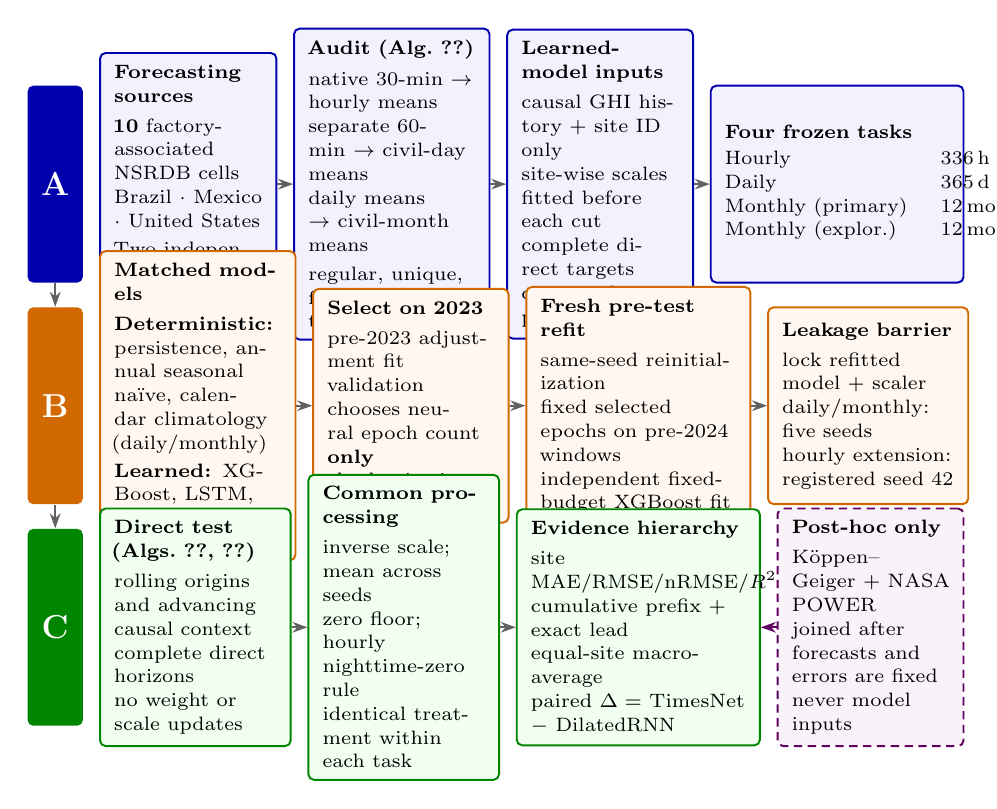
\begin{tikzpicture}[
  node distance=2mm,
  flow/.style={-{Stealth[length=1.9mm,width=1.35mm]},draw=black!62,line width=0.7pt},
  band label/.style={rounded corners=2pt,text=white,font=\bfseries\large,
    minimum width=7mm,minimum height=25mm,align=center,inner sep=1mm},
  flow box/.style={rounded corners=2pt,line width=0.7pt,align=left,
    minimum height=25mm,inner xsep=1.8mm,inner ysep=1.5mm,
    font=\fontsize{7.5}{8.6}\selectfont},
  a step/.style={flow box,draw=blue!68!black,fill=blue!5},
  b step/.style={flow box,draw=orange!82!black,fill=orange!6},
  c step/.style={flow box,draw=green!52!black,fill=green!6},
  external/.style={flow box,draw=violet!75!black,fill=violet!5,densely dashed},
  heading/.style={font=\fontsize{8.3}{9.2}\selectfont\bfseries}
]

% A — source audit and task construction.
\node[band label,fill=blue!68!black] (a-label) {A};
\node[a step,text width=0.155\textwidth,right=2mm of a-label] (sources) {
  {\bfseries Forecasting sources}\\[0.8mm]
  \textbf{10} factory-associated NSRDB cells\\
  Brazil $\cdot$ Mexico $\cdot$ United States\\[0.6mm]
  Two independent 2019--2024 archives
};
\node[a step,text width=0.175\textwidth,right=2mm of sources] (audit) {
  {\bfseries Audit (Alg.~\ref{alg:matched-training})}\\[0.8mm]
  native 30-min $\rightarrow$ hourly means\\
  separate 60-min $\rightarrow$ civil-day means\\
  daily means $\rightarrow$ civil-month means\\[0.6mm]
  regular, unique, finite, nonnegative series
};
\node[a step,text width=0.165\textwidth,right=2mm of audit] (contract) {
  {\bfseries Learned-model inputs}\\[0.8mm]
  causal GHI history + site ID only\\
  site-wise scales fitted before each cut\\
  complete direct targets contained in partition
};
\node[a step,text width=0.235\textwidth,right=2mm of contract] (tasks) {
  {\bfseries Four frozen tasks}\\[0.8mm]
  \begin{tabular}{@{}ll@{}}
    Hourly & $336\,\mathrm{h}\rightarrow72\,\mathrm{h}$\\
    Daily & $365\,\mathrm{d}\rightarrow30\,\mathrm{d}$\\
    Monthly (primary) & $12\,\mathrm{mo}\rightarrow1\,\mathrm{mo}$\\
    Monthly (explor.) & $12\,\mathrm{mo}\rightarrow6\,\mathrm{mo}$
  \end{tabular}
};
\draw[flow] (sources.east) -- (audit.west);
\draw[flow] (audit.east) -- (contract.west);
\draw[flow] (contract.east) -- (tasks.west);

% B — matched development and explicit leakage barrier.
\node[band label,fill=orange!82!black,below=3mm of a-label] (b-label) {B};
\node[b step,text width=0.175\textwidth,right=2mm of b-label] (models) {
  {\bfseries Matched models}\\[0.8mm]
  \textbf{Deterministic:} persistence, annual seasonal na\"ive, calendar climatology (daily/monthly)\\[0.5mm]
  \textbf{Learned:} XGBoost, LSTM, TimesNet, DilatedRNN
};
\node[b step,text width=0.175\textwidth,right=2mm of models] (selection) {
  {\bfseries Select on 2023}\\[0.8mm]
  pre-2023 adjustment fit\\
  validation chooses neural epoch count \textbf{only}\\
  checkpoint is discarded
};
\node[b step,text width=0.205\textwidth,right=2mm of selection] (refit) {
  {\bfseries Fresh pre-test refit}\\[0.8mm]
  same-seed reinitialization\\
  fixed selected epochs on pre-2024 windows\\
  independent fixed-budget XGBoost fit
};
\node[b step,text width=0.18\textwidth,right=2mm of refit] (lock) {
  {\bfseries Leakage barrier}\\[0.8mm]
  lock refitted model + scaler\\
  daily/monthly: five seeds\\
  hourly extension: registered seed 42
};
\draw[flow] (models.east) -- (selection.west);
\draw[flow] (selection.east) -- (refit.west);
\draw[flow] (refit.east) -- (lock.west);

% C — frozen test, common processing, and evidence hierarchy.
\node[band label,fill=green!52!black,below=3mm of b-label] (c-label) {C};
\node[c step,text width=0.17\textwidth,right=2mm of c-label] (test) {
  {\bfseries Direct test (Algs.~\ref{alg:timesnet-direct}, \ref{alg:dilated-direct})}\\[0.8mm]
  rolling origins and advancing causal context\\
  complete direct horizons\\
  no weight or scale updates
};
\node[c step,text width=0.17\textwidth,right=2mm of test] (physics) {
  {\bfseries Common processing}\\[0.8mm]
  inverse scale; mean across seeds\\
  zero floor; hourly nighttime-zero rule\\
  identical treatment within each task
};
\node[c step,text width=0.225\textwidth,right=2mm of physics] (evidence) {
  {\bfseries Evidence hierarchy}\\[0.8mm]
  site MAE/RMSE/nRMSE/$R^2$\\
  cumulative prefix + exact lead\\
  equal-site macro-average\\
  paired $\Delta=$ TimesNet $-$ DilatedRNN
};
\node[external,text width=0.165\textwidth,right=2mm of evidence] (context) {
  {\bfseries Post-hoc only}\\[0.8mm]
  K\"oppen--Geiger + NASA POWER\\
  joined after forecasts and errors are fixed\\
  never model inputs
};
\draw[flow] (test.east) -- (physics.west);
\draw[flow] (physics.east) -- (evidence.west);
\draw[-{Stealth[length=1.9mm,width=1.35mm]},draw=violet!75!black,
  densely dashed,line width=0.7pt] (context.west) -- (evidence.east);

\draw[flow] (a-label.south) -- (b-label.north);
\draw[flow] (b-label.south) -- (c-label.north);

\end{tikzpicture}
\caption{End-to-end matched forecasting design. (A) Independent NSRDB archives
are audited and converted into four direct-output tasks; learned models
receive causal GHI and site identity. (B) Model selection and fresh pre-test
refitting follow Algorithm~\ref{alg:matched-training}. (C) Direct test
forecasts from Algorithms~\ref{alg:timesnet-direct} and
\ref{alg:dilated-direct} receive common physical
post-processing before location-first aggregation and paired comparison;
K\"oppen--Geiger and NASA POWER fields enter only after errors are fixed.}
\label{fig:pipeline}
\end{figure*}


\subsubsection{Block A: data contract and temporal windows}

Block A establishes the information set before any model is fitted. It audits
the regular series, applies the task resolution, assigns a stable site
identifier, creates the chronological partitions, and fits two independent
sets of site-wise min--max parameters. The selection scale contains only
observations before 2023, whereas the refit scale contains only observations
before 2024.

The resulting sample has the input defined in Eq.~\eqref{eq:matched_input}.
A timestamp determines availability and alignment but is not presented as a
feature for the learned models. Likewise, latitude, longitude, climate class,
NASA POWER variables, and explicit calendar covariates are excluded from their
inputs. Holding this information set constant controls feature availability
in the learned-model comparison. Seasonal references additionally use known
calendar labels, as specified below.

\subsubsection{Block B: matched model development}

The deterministic references are persistence, annual seasonal na\"ive, and
calendar climatology, with resolution-specific definitions. In the hourly
task, daily-profile persistence repeats the last 24 observed local hours
cyclically across the 72-hour output; the annual seasonal baseline retrieves the
same local hour one year earlier. In the daily and monthly tasks, persistence
repeats the most recent daily or monthly aggregate throughout the output, and
the annual baseline retrieves the same civil day or month one year earlier.
Every annual reference is asserted to precede the forecast origin, with
29 February mapped to 28 February. Daily and monthly climatology averages each
calendar day or month separately at each site, using only values before the
relevant cut. The official hourly artifact contains persistence and annual
seasonal na\"ive forecasts; it does not contain calendar climatology.
These references use the same GHI archive, but their calendar lookup and
pre-cut historical summaries are not restricted to the learned models'
lag-vector representation.

The learned comparison comprises XGBoost, a direct LSTM, TimesNet, and a direct
DilatedRNN. These models share the scaled GHI sequence and site identifier;
neural models encode the identifier with a learned embedding, whereas XGBoost
uses a one-hot representation. TimesNet selects its Fourier periods separately
for every input window; consequently, other windows in an inference batch
cannot alter its periods or forecast. Each learned model--seed instance is
fitted globally across sites, sharing parameters while retaining site identity
\cite{montero2021}. Every multi-step model produces the complete target vector
in one forward pass, so no predicted GHI is recursively returned as input.

Reinitialization is mandatory: the validation checkpoint is not continued into
the test fit. For neural models, 2023 selects only the number of epochs for each
model--seed pair. The final instance is trained from a fresh initialization on
all declared pre-test windows for exactly that number of epochs. XGBoost has a
fixed tree budget and is independently fitted on the adjustment and refit
partitions. The hourly extension is narrower: all official model forecasts are
read without modification, and only DilatedRNN with seed 42 is added and
aligned by site, origin, target timestamp, and lead.

\begin{algorithm}[!htbp]
\caption{Matched TimesNet--DilatedRNN preparation and refit}
\label{alg:matched-training}
\footnotesize
\begin{algorithmic}[1]
\Require Task $(r,C,H)$; site archives; fixed cutoffs and settings
\Ensure Origin-aligned TimesNet and DilatedRNN forecasts and metrics
\State Load the archive for $r$; audit the common time grid and GHI
\State For monthly tasks, average audited daily values by civil month
\State Build initial training (adjustment) windows $\mathcal W_A$
\Statex \hspace{\algorithmicindent}and validation $\mathcal W_V$, refit $\mathcal W_R$, and test $\mathcal W_T$ windows
\Statex \hspace{\algorithmicindent}with context $y_{t-C:t-1}$, targets $y_{t:t+H-1}$, and site ID
\State Reject target windows crossing a cutoff; verify origin counts
\State Fit site scales $S_A$ before 2023 and $S_R$ before 2024
\If{hourly extension}
  \State Verify hashes; load the official TimesNet seed-42 forecasts
  \State $\mathcal M\gets\{\mathrm{DilatedRNN}\}$; $\mathcal S\gets\{42\}$
\Else
  \State $\mathcal M\gets\{\mathrm{TimesNet,DilatedRNN}\}$
  \State $\mathcal S\gets\{11,23,42,67,89\}$
\EndIf
\For{each $(m,s)\in\mathcal M\times\mathcal S$}
  \State Initialize with $s$; fit $S_A(\mathcal W_A)$ using Adam
  \State Select $E^\star$ by early stopping on $S_A(\mathcal W_V)$ MSE
  \State Retain the validation forecasts from epoch $E^\star$
  \State Discard weights; reinitialize with the same seed $s$
  \State Fit $S_R(\mathcal W_R)$ for exactly $E^\star$ epochs
  \State Forecast every $S_R(\mathcal W_T)$ context with fixed weights
  \Statex \hspace{\algorithmicindent}(Algorithms~\ref{alg:timesnet-direct} and \ref{alg:dilated-direct})
  \State Invert $S_A$ for validation and $S_R$ for test forecasts
  \State Retain the unbounded seed forecasts in W/m$^2$
\EndFor
\State For daily/monthly tasks, average raw forecasts across seeds
\State Post-process each new seed and ensemble forecast:
\Statex \hspace{\algorithmicindent}apply the zero floor and, if hourly, the nighttime mask
\State Verify common $(\ell,t,\mathrm{lead},\mathrm{target})$ keys
\State Compute site metrics, then macro summaries with equal site weights
\end{algorithmic}
\end{algorithm}


All partitions are evaluated in rolling-origin form. Model parameters and the
refit scale remain fixed throughout the 2024 test, but the causal context is
advanced at every eligible origin and may include GHI observations from earlier
in 2024 once they have become historical. No test target enters a context before
its timestamp, and no weights are updated during the test. The design is thus a
retrospective walk-forward evaluation with fixed parameters, not a single
forecast issued at the end of 2023 for every target in 2024.

\FloatBarrier
\subsubsection{Direct architecture implementations}

Algorithm~\ref{alg:timesnet-direct} specifies the compact TimesNet forward
pass used in the comparison. The site-scaled context is standardized within
the current window, embedded with position and site identity, and processed
using periods selected separately for that sample. After the TimesBlock,
a direct temporal projection maps the context to the complete forecast
horizon. The final step restores the external site-normalized scale; the
common physical post-processing is applied later in Block C.

\begin{algorithm}[!htbp]
\caption{Direct forward pass of the compact TimesNet}
\label{alg:timesnet-direct}
\footnotesize
\begin{algorithmic}[1]
\Require Fitted TimesNet; scaled context $\mathbf x$; site $\ell$
\Ensure $H$ predictions in the external site-normalized scale
  \State $\mu\gets\operatorname{mean}(\mathbf x)$;
  $\sigma\gets\sqrt{\operatorname{var}_{\mathrm{pop}}(\mathbf x)+10^{-5}}$
  \State $\mathbf u\gets(\mathbf x-\mu)/\sigma$
  \State $\mathbf Z\gets\mathrm{ValueEmbed}(\mathbf u)+\mathrm{PositionEmbed}$
  \State $\mathbf Z\gets\mathbf Z+\mathrm{SiteEmbed}(\ell)$
  \State Apply embedding dropout during training only
  \For{each TimesBlock}
    \State Compute FFT amplitudes separately for this sample
    \State Select the top-$k$ nonzero frequencies $f_i$
    \For{each selected $f_i$}
      \State $p_i\gets\lfloor C/f_i\rfloor$
      \State Pad and fold $\mathbf Z$ into cycles of length $p_i$
      \State Apply the two-layer Inception convolution with GELU
      \State Unfold and trim to $C$ steps, obtaining $\mathbf U_i$
    \EndFor
    \State $\alpha_i\gets\mathrm{softmax}_i(\mathrm{FFTAmplitude}(f_i))$
    \State $\mathbf Z\gets\mathrm{LayerNorm}(\mathbf Z+\sum_i\alpha_i\mathbf U_i)$
  \EndFor
  \State $\mathbf F\gets\mathrm{TemporalProject}_{C\to H}(\mathbf Z)$
  \State $\widehat{\mathbf u}\gets\mathrm{ChannelProject}(\mathbf F)$
  \State \Return $\sigma\widehat{\mathbf u}+\mu$
\end{algorithmic}
\end{algorithm}


Algorithm~\ref{alg:dilated-direct} specifies the alternative recurrent path.
Each layer shares its tanh-RNN weights across residue chains with the same
dilation, then reassembles the outputs in temporal order. The last state
and the site embedding feed a direct output head. The explicit forward
passes make clear which operations differ while both architectures retain
the same context, site identity, target vector, and subsequent evaluation.

\begin{algorithm}[H]
\caption{Direct forward pass of the DilatedRNN}
\label{alg:dilated-direct}
\footnotesize
\begin{algorithmic}[1]
\Require Fitted DilatedRNN; site-scaled $\mathbf x\in\mathbb R^{C\times1}$; site $\ell$
\Ensure $H$ predictions in the external site-normalized scale
  \State $\mathbf Z\gets\mathbf x$
  \For{each dilation $d\in(1,2,4)$}
    \State Use this layer's shared 16-unit tanh-RNN
    \State Process $\mathbf Z_{j,j+d,\ldots}$ from zero states, $0\leq j<d$
    \State $\mathbf Z\gets$ outputs in time order, of shape $C\times16$
  \EndFor
  \State $\mathbf v\gets[\mathbf Z_{C-1};\mathrm{SiteEmbed}(\ell)]\in\mathbb R^{24}$
  \State $\mathbf a\gets\mathrm{ReLU}(\mathrm{Linear}_{24\to16}(\mathbf v))$
  \State \Return $\mathrm{Linear}_{16\to H}(\mathbf a)$
\end{algorithmic}
\end{algorithm}


\subsubsection{Block C: physical consistency and evaluation}

For daily and monthly learned models, the ensemble is the arithmetic mean
of the five inverse-scaled forecasts before physical post-processing.
If $\widetilde{y}^{(s)}$ is the unbounded forecast in W/m$^2$ from seed $s$,
the reported ensemble forecast is
\begin{equation}
 \widehat{y}^{\mathrm{ens}}
 =
 \max\!\left(0,\frac{1}{5}\sum_{s=1}^{5}\widetilde{y}^{(s)}\right).
 \label{eq:ensemble_forecast}
\end{equation}
Seed-level forecasts receive their own zero floor before their metrics are
computed. Averaging forecasts and averaging their errors are distinct
operations.

All forecasts receive the same non-negativity floor after inverse scaling.
Daily and monthly forecasts have no upper truncation. Hourly forecasts also use
solar elevation computed at the centre of each hourly interval; predictions
are set to zero when elevation is nonpositive, following the deterministic
geometry implemented with \texttt{pvlib} \cite{anderson2023}. Solar elevation
is therefore a post-processing constraint, not privileged predictive
information.

The unit of the matched descriptive comparison is the location. For each
metric and horizon scope, the pipeline retains the TimesNet--DilatedRNN
difference, its mean and median across the ten sites, and the number of sites
won by TimesNet. It does not treat overlapping forecast origins as independent
replicates. The NASA POWER join occurs only in the final interpretive layer,
using the predeclared operational 1~mm/day and 80\% thresholds from
Section~\ref{sec:data}; it cannot influence training, model selection, or the
reported aggregate metrics.

\FloatBarrier
\subsection{Experimental Setup}
\label{sec:experiments}

The executable study defines the four frozen tasks in Band A of
Figure~\ref{fig:pipeline} rather than comparing errors across unlike
resolutions. Their complete contexts, outputs, evaluation horizons, and origin
counts are retained in the Supplementary Material. Within a task, all models
share sites, origins, targets, fitting cuts, and post-processing. Across tasks,
MAE and RMSE retain W/m$^2$ units but refer to different temporal aggregates;
they are not pooled.

\subsubsection{Common matched protocol}

The daily and monthly experiments contain three deterministic references
(persistence, annual seasonal na\"ive, and calendar climatology) and four
learned models (XGBoost, LSTM, TimesNet, and DilatedRNN). Every learned
model receives only causal GHI and site identity. Neural models use the five
seeds 11, 23, 42, 67, and 89, and XGBoost is likewise refitted under each of
those seeds because row and column subsampling are stochastic; both seed-level
forecasts and the arithmetic mean of every learned model are retained.
Deterministic references are evaluated once. The primary model comparison uses
macro-MAE after computing
MAE separately at each site. RMSE, nRMSE, and $R^2$, as well as cumulative and
exact-lead scopes, remain mandatory complementary outputs.

For selection, neural networks are initialized under each seed, fitted to the
adjustment windows, and monitored on the 2023 windows using normalized MSE.
Early stopping chooses an epoch count for each model--seed pair. The network is
then discarded, reinitialized under the same seed, and fitted to the pre-2024
refit windows for exactly that number of epochs. Thus, epoch selection
minimizes validation MSE in site-normalized units, while the reported primary
ranking uses test MAE in physical units. XGBoost uses its frozen tree
budget in separate adjustment and refit instances. Test forecasts are generated
only by the refitted instances.

Band B of Figure~\ref{fig:pipeline} summarizes this selection--refit chronology;
Band A shows the four direct-output contracts that remain fixed during testing.

Within each partition, forecasts follow the rolling-origin protocol of
Section~\ref{sec:methodology}: the official hourly task advances one local-
midnight origin per day, the daily task advances one origin per day, and the
monthly tasks advance one origin per civil month. Parameters remain fixed in
the test partition while each context incorporates only observations that have
become available before its first target.

\subsubsection{Hourly protocol and DilatedRNN extension}

The official hourly task uses 336 past hours (14 days) and produces the next
72 hours directly. The reported checkpoints are 24, 48, and 72 hours; they are
prefixes and exact leads extracted from the same 72-hour output, not separately
trained models. Adjustment origins run from 15 January 2019 through
29 December 2022 (1,445 per site), and validation origins run from
1 January through 29 December 2023 (363 per site). The pre-test refit combines
origins from 15 January 2019 through 29 December 2023 (1,810 per site). The
retrospective test contains 363 origins from 1 January through
28 December 2024. The last 72-hour window ends at 23:00 on 30 December in the
fixed local-time index; corresponding UTC timestamps can extend into
31 December for western locations.

The official artifact fixes seed 42 and contains persistence, annual seasonal
na\"ive, XGBoost, LSTM, and TimesNet predictions. The extension trains only a
direct DilatedRNN with seed 42 under the same 336-to-72 contract. Its forecasts
are merged one-to-one with the read-only official artifact by site, forecast
origin, target timestamp, and lead. Target equality is checked during the
one-to-one merge, and the hashes of all official inputs are rechecked before
the extension is marked complete. Thus the hourly extension does not silently
retrain or overwrite an official comparator.

\subsubsection{Daily protocol}

The daily primary task uses 365 daily means to predict a 30-day vector. Metrics
are retained at 1, 3, 7, 14, and 30 days. Adjustment origins extend from
1 January 2020 through 2 December 2022, with targets ending no later than
31 December 2022 (1,067 origins per site). Validation uses
1 January--2 December 2023 (336 origins), and refit uses
1 January 2020--2 December 2023 (1,432 origins). The 2024 test uses
1 January--2 December and contains 337 complete origins per site because 2024
is a leap year.

\subsubsection{Monthly primary and exploratory protocols}

Civil-month means are calculated from the audited daily series. The primary
monthly task uses 12 months to predict the next month. It has 36 adjustment
origins in 2020--2022, 12 validation origins in 2023, 48 refit origins in
2020--2023, and 12 test origins in 2024, for every site.

The exploratory monthly task uses the same 12-month context and directly
predicts six months. Its declared checkpoints are months 1, 3, and 6.
The final origin in each partition must fall no later than July so that all
six targets remain inside its final year. Adjustment therefore contains
31 consecutive monthly origins from January 2020 through July 2022, validation
contains seven from January through July 2023, refit contains 43 from January
2020 through July 2023, and test contains seven from January through July 2024.
Earlier complete years in adjustment and refit retain all twelve origins.
This task is explicitly labelled exploratory because each site contributes
only seven test origins, each with a six-month output.

For the six-month task, exact leads are evaluated on different target-month
sets: lead 1 covers January--July, whereas lead 6 covers June--December. Its
horizon profile therefore combines lead-time and seasonal effects and is not
interpreted as an isolated degradation curve.

\subsubsection{Frozen optimization settings}

Table~\ref{tab:hyperparameters} gives the compact configuration needed to
interpret the main comparison. The Supplementary Material records the
full temporal boundaries, model settings, baseline definitions, artifact
contract, and external-context integrity hashes.

\begin{table}[!t]
\centering
\caption{Compact fixed configuration of the matched implementation.}
\label{tab:hyperparameters}
\footnotesize
\setlength{\tabcolsep}{3pt}
\renewcommand{\arraystretch}{1.12}
\begin{tabular}{@{}
  >{\raggedright\arraybackslash}p{0.27\linewidth}
  >{\raggedright\arraybackslash}p{0.66\linewidth}@{}}
\toprule
\textbf{Component} & \textbf{Fixed setting} \\
\midrule
Matched input & Causal GHI sequence plus fixed site identifier only \\
Regression/output & Continuous GHI; direct vector of task-specific length \\
Neural optimization & Adam; MSE loss; learning rate $10^{-3}$;
weight decay $10^{-5}$ \\
Batch size & 128 for hourly/daily; 32 for monthly \\
Epoch selection & Hourly/daily: maximum 30, patience 5; monthly:
maximum 300, patience 30 \\
Seeds & Daily/monthly: 11, 23, 42, 67, 89; official hourly and
DilatedRNN extension: 42 \\
TimesNet & $d_{\mathrm{model}}=8$, $d_{\mathrm{ff}}=16$, one TimesBlock,
top-$k=3$, two kernels, dropout 0.1 \\
DilatedRNN & Dilations $(1,2,4)$; 16 units/layer; dense width 16;
dropout 0 \\
LSTM & One layer; hidden width 32; direct output head \\
Site embedding & Width 8 for all neural models \\
XGBoost & 150 trees; depth 3; learning rate 0.05; row and column
subsampling 0.8; histogram tree method \\
Post-processing & Zero floor for all tasks; hourly values also set to zero
when solar elevation is nonpositive \\
\bottomrule
\end{tabular}
\end{table}


\subsubsection{Model capacity and computational evidence}

To make differences in model capacity explicit,
Table~\ref{tab:model_capacity} gives the exact number of trainable scalar
parameters in each neural model. The counts are obtained from the frozen module
dimensions, including biases and the ten-site embedding, rather than inferred
from checkpoint file sizes. TimesNet has a task-dependent direct temporal
projection, so its parameter count grows with both context and output length.
Dilated recurrence changes the temporal connections without adding separate
weights for each skipped position. XGBoost is instead constrained by 150 trees
of maximum depth three and is not assigned an artificial neural-parameter
equivalent.

\input{tables/model_capacity}

Training and inference times were not measured consistently across the
completed runs. The computational comparison therefore reports parameter
counts and the common one-thread policy; runtime comparisons remain for
future evaluation.

\subsection{Evaluation Metrics}
\label{sec:metrics}

Let $y_i$ be a reference GHI value, $\widehat{y}_i$ its post-processed
forecast, $e_i=y_i-\widehat{y}_i$, $\bar{y}$ the mean reference value in the
same evaluation vector, and $n$ its number of origin--lead forecast pairs.
A target timestamp can therefore occur more than once when it is predicted
from different origins. Each metric is
computed first for one site, one model estimate, one partition, one declared
horizon, and one horizon scope.

\subsubsection{Mean absolute error}

\begin{equation}
 \mathrm{MAE}
 =
 \frac{1}{n}\sum_{i=1}^{n}\left|e_i\right|.
 \label{eq:mae}
\end{equation}
MAE is the primary error measure and remains in W/m$^2$. Its linear penalty
makes the magnitude directly interpretable and less dominated by individual
large deviations than a squared-error score \cite{hyndman2006}. Lower values
are better.

\subsubsection{Root mean squared error}

\begin{equation}
 \mathrm{RMSE}
 =
 \sqrt{\frac{1}{n}\sum_{i=1}^{n}e_i^2}.
 \label{eq:rmse}
\end{equation}
RMSE is also expressed in W/m$^2$, but squaring gives larger deviations more
weight. Reporting it alongside MAE reveals whether occasional large errors
change the model ordering, a standard concern in deterministic solar-forecast
verification \cite{yang2020verification}. Lower values are better.

\subsubsection{Normalized root mean squared error}

\begin{equation}
 \mathrm{nRMSE}
 =
 \frac{\mathrm{RMSE}}{\bar{y}},
 \qquad
 \mathrm{nRMSE}_{\%}=100\,\mathrm{nRMSE}.
 \label{eq:nrmse}
\end{equation}
The machine-readable artifacts store the dimensionless ratio; tables that use
percent explicitly multiply it by 100. Normalization supports comparison among
sites with different mean irradiance levels, but it inherits the instability
of a small denominator \cite{voyant2022}. The value is therefore left undefined
when $\bar{y}$ is numerically zero. Lower values are better.

\subsubsection{Coefficient of determination}

\begin{equation}
 R^2
 =
 1-
 \frac{\sum_{i=1}^{n}e_i^2}
      {\sum_{i=1}^{n}(y_i-\bar{y})^2}.
 \label{eq:r2}
\end{equation}
$R^2$ measures variation tracked relative to a constant predictor built from
the evaluation mean \cite{yang2020verification}. It is undefined for fewer
than two targets or a constant reference vector and can be negative when the
forecast is worse than that constant reference. Higher values are better;
$R^2$ does not replace the scale-dependent errors.

\subsubsection{Horizon scopes and spatial aggregation}

For a declared horizon $H$, the cumulative scope concatenates leads
$1,\ldots,H$ over all valid origins, whereas the exact-lead scope retains only
lead $H$. The two scopes are identical at $H=1$. This distinction is applied at
24, 48, and 72 hours; 1, 3, 7, 14, and 30 days; and, for the exploratory
multi-month task, 1, 3, and 6 months. A horizon label therefore always denotes
both a numerical lead and an explicitly named scope. The main rankings use
the cumulative scope.

Hourly origins are fixed at local midnight, so exact leads 24, 48, and 72
all select the 23:00 interval on their respective target days. In this test
set these nighttime targets and post-processed forecasts are zero: exact-lead
MAE and RMSE are zero for every model, while nRMSE and $R^2$ are undefined.
They are retained as audit outputs and do not measure daytime forecast skill.

Within each site, cumulative metrics weight origin--lead pairs equally,
including repeated forecasts for a shared target timestamp. They therefore
evaluate the issued forecast trajectories rather than one unique forecast
per calendar time. Target periods inside an overlapping window can receive
more contributions than periods near the test boundaries.

Let $\mathcal{L}_{M}$ be the set of locations with a finite site-level value
of metric $M$, and let $L_M=|\mathcal{L}_{M}|$. The macro result is
\begin{equation}
 M_{\mathrm{macro}}
 =
 \frac{1}{L_M}\sum_{\ell\in\mathcal{L}_{M}}M_{\ell},
 \qquad L_M>0.
 \label{eq:macro_metric}
\end{equation}
Undefined site-level values are excluded from the corresponding mean; if
none are finite, the macro value remains undefined. All ten sites contribute
to the main cumulative results. Equal site weighting prevents a site with more
valid forecast pairs from dominating the geographical summary.
Macro-MAE is the predeclared primary
metric at every resolution; MAE, RMSE, nRMSE, and $R^2$ are nevertheless
retained together rather than selectively reported.

For daily and monthly learned models, seed-level metrics describe variability
across five fitted instances on the same test data. Their standard deviation
measures sensitivity to the registered seeds; it is neither a forecast
prediction interval nor a confidence interval for generalization error.
The TimesNet--DilatedRNN paired comparison uses the post-processed five-seed
ensemble forecast from Eq.~\eqref{eq:ensemble_forecast}. The hourly extension compares the single
registered seed 42 for both models. For each site, metric, horizon, and scope,
the pipeline stores
\begin{equation}
 \Delta_{\ell,M}
 =
 M_{\ell,\mathrm{TimesNet}}-M_{\ell,\mathrm{DilatedRNN}}.
 \label{eq:paired_difference}
\end{equation}
A negative $\Delta_{\ell,M}$ is a TimesNet win for the three error metrics; a
positive value is a win for $R^2$. Mean and median differences and the number
of site wins are descriptive. Overlapping multi-step windows are not treated
as independent observations for an i.i.d. significance test.


\section{Results and Discussion}
\label{sec:results}

\subsection{Primary architecture comparison}

Table~\ref{tab:architecture_winners} identifies the lower-MAE architecture
at every cumulative checkpoint. All values are equal-site-weighted test
macro-MAEs, computed from the same origins and targets within each task.
Daily and monthly values evaluate the five-seed forecast ensemble; hourly
values evaluate the registered seed 42. A cumulative horizon includes all
leads up to that checkpoint, rather than only the final lead.

At the terminal horizons, TimesNet led the 72-hour task, with
52.48 versus 52.96~W/m$^2$ for DilatedRNN. DilatedRNN led the 30-day task
(43.85 versus 44.08~W/m$^2$), the principal one-month task
(13.01 versus 13.89~W/m$^2$), and the exploratory six-month task
(14.37 versus 14.46~W/m$^2$). Thus, the terminal winner was TimesNet for
the hourly contract and DilatedRNN for the daily and monthly contracts.
The largest relative terminal reduction was the one-month DilatedRNN gain:
6.38\% relative to TimesNet, calculated from unrounded MAEs. Counting these
four wins does not define an overall score because the targets, forecast
origins, and aggregation scales differ across tasks.

\begin{table*}[!t]
\centering
\caption{Focused architecture comparison: cumulative test macro-MAE in W/m$^2$. Bold marks the lower unrounded MAE within each row. $\Delta=\mathrm{MAE}_{\mathrm{TimesNet}}-\mathrm{MAE}_{\mathrm{DilatedRNN}}$ is computed before rounding. Hourly estimates use seed 42; daily and monthly estimates use five-seed ensembles. The complete reference-model benchmark is retained in Supplementary Table S1.}
\label{tab:architecture_winners}
\small
\setlength{\tabcolsep}{5pt}
\begin{tabular}{llrrrl}
\toprule
Task & Cumulative horizon & TimesNet & DilatedRNN & $\Delta$ & Lower MAE \\
\midrule
Hourly & 24 h & \textbf{49.39} & 50.73 & -1.35 & TimesNet \\
Hourly & 48 h & 52.16 & \textbf{52.15} & +0.02 & DilatedRNN \\
Hourly & 72 h & \textbf{52.48} & 52.96 & -0.48 & TimesNet \\
\addlinespace
Daily & 1 d & \textbf{43.20} & 43.27 & -0.07 & TimesNet \\
Daily & 3 d & \textbf{43.63} & 43.80 & -0.17 & TimesNet \\
Daily & 7 d & \textbf{43.95} & 44.08 & -0.13 & TimesNet \\
Daily & 14 d & \textbf{44.09} & 44.11 & -0.02 & TimesNet \\
Daily & 30 d & 44.08 & \textbf{43.85} & +0.23 & DilatedRNN \\
\addlinespace
Monthly 12--1 & 1 mo & 13.89 & \textbf{13.01} & +0.89 & DilatedRNN \\
\addlinespace
Monthly 12--6 & 1 mo & \textbf{14.86} & 14.89 & -0.03 & TimesNet \\
Monthly 12--6 & 3 mo & 14.49 & \textbf{14.33} & +0.16 & DilatedRNN \\
Monthly 12--6 & 6 mo & 14.46 & \textbf{14.37} & +0.09 & DilatedRNN \\
\bottomrule
\end{tabular}
\end{table*}


Table~\ref{tab:metricas-terminais} complements MAE with RMSE, nRMSE, and
$R^2$. The terminal RMSE ordering agrees with the MAE ordering: at 72 hours,
TimesNet obtained 101.17~W/m$^2$ versus 104.93~W/m$^2$ for DilatedRNN;
DilatedRNN had the lower RMSE in the daily and monthly tasks. These are
matched-test results, and their role is to resolve the architecture
comparison under the specified protocol. Results against all other
evaluated models are retained in the Supplementary Material and discussed
in Section~\ref{sec:reference_benchmark}.

\begin{table*}[htbp]
\centering
\caption{Terminal cumulative metrics for TimesNet and DilatedRNN. MAE and RMSE are in W/m$^2$; nRMSE is reported as a percentage.}
\label{tab:metricas-terminais}
\small
\setlength{\tabcolsep}{5pt}
\begin{tabular}{ll l rrrr}
\toprule
Task & Horizon & Model & MAE & RMSE & nRMSE (\%) & $R^2$ \\
\midrule
Hourly 336--72 & 72 h & TimesNet & 52.48 & 101.17 & 50.41 & 0.87 \\
Hourly 336--72 & 72 h & DilatedRNN & 52.96 & 104.93 & 52.31 & 0.86 \\
\addlinespace
Daily 365--30 & 30 d & TimesNet & 44.08 & 55.16 & 26.55 & 0.53 \\
Daily 365--30 & 30 d & DilatedRNN & 43.85 & 54.79 & 26.38 & 0.54 \\
\addlinespace
Monthly 12--1 & 1 mo & TimesNet & 13.89 & 17.49 & 8.51 & 0.88 \\
Monthly 12--1 & 1 mo & DilatedRNN & 13.01 & 16.02 & 7.86 & 0.91 \\
\addlinespace
Monthly 12--6 & 6 mo & TimesNet & 14.46 & 18.24 & 7.77 & 0.85 \\
Monthly 12--6 & 6 mo & DilatedRNN & 14.37 & 17.47 & 7.47 & 0.85 \\
\bottomrule
\end{tabular}
\end{table*}


\subsection{Site-paired differences and horizon dependence}

Table~\ref{tab:vitorias-timesnet-dilatedrnn} gives the site-paired comparison;
a negative difference denotes lower TimesNet MAE. TimesNet led at 24 and
72 hours by 1.35 and 0.48~W/m$^2$, respectively; DilatedRNN led at 48 hours
by 0.02~W/m$^2$. Differences are calculated before rounding individual
MAEs. TimesNet won seven sites at 24 hours and four at both 48 and 72 hours.
Its 72-hour macro advantage therefore reflects the magnitude of local gains,
even though DilatedRNN won more sites.

In the daily task, TimesNet led by 0.07--0.17~W/m$^2$ through seven days and
by 0.02~W/m$^2$ at 14 days. At 30 days, DilatedRNN led by
0.23~W/m$^2$ and won six sites. DilatedRNN also led the principal one-month
task by 0.89~W/m$^2$ and won six sites. In the exploratory six-month task,
TimesNet led the one-month prefix by 0.03~W/m$^2$ despite winning only four
sites. DilatedRNN led by 0.16 and 0.09~W/m$^2$ at three and six months,
respectively, and won seven sites at the terminal horizon. At three months,
TimesNet won six sites despite its higher macro-MAE. These reversals show
why both the magnitude and the distribution of site-level errors matter.

\begin{table*}[htbp]
\centering
\caption{Descriptive site-paired cumulative comparison. $\Delta=\mathrm{MAE}_{\mathrm{TimesNet}}-\mathrm{MAE}_{\mathrm{DilatedRNN}}$ in W/m$^2$; negative values favor TimesNet (TN), positive values favor DilatedRNN (DR). Wins count sites, not forecast origins. Overlapping multi-step targets are not independent observations.}
\label{tab:vitorias-timesnet-dilatedrnn}
\small
\setlength{\tabcolsep}{5pt}
\begin{tabular*}{\textwidth}{@{\extracolsep{\fill}}llrrrrrr@{}}
\toprule
Task & Horizon & Sites & Mean $\Delta$ & Median $\Delta$ & TN wins & DR wins & Ties \\
\midrule
Hourly 336--72 & 24 h & 10 & -1.35 & -1.33 & 7 & 3 & 0 \\
Hourly 336--72 & 48 h & 10 & 0.02 & 0.62 & 4 & 6 & 0 \\
Hourly 336--72 & 72 h & 10 & -0.48 & 0.50 & 4 & 6 & 0 \\
\addlinespace
Daily 365--30 & 1 d & 10 & -0.07 & -0.04 & 5 & 5 & 0 \\
Daily 365--30 & 3 d & 10 & -0.17 & -0.15 & 5 & 5 & 0 \\
Daily 365--30 & 7 d & 10 & -0.13 & -0.23 & 6 & 4 & 0 \\
Daily 365--30 & 14 d & 10 & -0.02 & -0.09 & 6 & 4 & 0 \\
Daily 365--30 & 30 d & 10 & 0.23 & 0.09 & 4 & 6 & 0 \\
\addlinespace
Monthly 12--1 & 1 mo & 10 & 0.89 & 0.35 & 4 & 6 & 0 \\
\addlinespace
Monthly 12--6 & 1 mo & 10 & -0.03 & 0.38 & 4 & 6 & 0 \\
Monthly 12--6 & 3 mo & 10 & 0.16 & -0.08 & 6 & 4 & 0 \\
Monthly 12--6 & 6 mo & 10 & 0.09 & 0.50 & 3 & 7 & 0 \\
\bottomrule
\end{tabular*}
\end{table*}


Figure~\ref{fig:local_heterogeneity} retains all ten terminal site contrasts.
The mixed signs show geographic heterogeneity and identify the locations at
which the task-level winner loses. They do not support a universal
architecture ranking.

\begin{figure*}[!t]
\centering
\includegraphics[width=0.90\textwidth]{heterogeneidade_local_delta_mae.png}
\caption{Site-level terminal cumulative contrast
$\Delta\mathrm{MAE}=\mathrm{MAE}_{\mathrm{TimesNet}}-
\mathrm{MAE}_{\mathrm{DilatedRNN}}$ in W/m$^2$. Negative (blue) cells
favor TimesNet; positive (red) cells favor DilatedRNN. Columns correspond to
72~h, 30~d, 1~month, and 6~months. Comparisons are descriptive; overlapping
multi-step target windows are not treated as independent observations.}
\label{fig:local_heterogeneity}
\end{figure*}

\subsection{Variability across seeds}

Daily and monthly learned models use five registered random seeds.
The 30-day seed-level macro-MAE was $44.29\pm0.29$~W/m$^2$ for TimesNet
and $44.10\pm0.60$~W/m$^2$ for DilatedRNN. At one month it was
$14.62\pm0.74$ versus $13.45\pm0.35$~W/m$^2$, respectively; at six months,
$15.24\pm0.76$ versus $14.77\pm0.45$~W/m$^2$.
Figure~\ref{fig:seed_variability} reports means and sample standard
deviations. These statistics need not equal
Table~\ref{tab:architecture_winners}: the latter evaluates the ensemble
forecast, whereas the former averages separately evaluated seed forecasts.
The hourly estimate uses one seed and cannot quantify seed variability.

The 0.23~W/m$^2$ terminal daily ensemble gap is smaller than either
architecture's seed-level standard deviation; the six-month gap is only
0.09~W/m$^2$. Comparing runs with the same seed, DilatedRNN had lower
terminal MAE in three of five daily runs and four of five runs in each
monthly task. The one-month advantage is thus more consistent across the
retained initializations, but is not universal. Seed standard deviations
measure training variability on the same test year; they are neither
confidence intervals nor estimates of uncertainty across future years.
Comparing an ensemble gap with these deviations is descriptive, not a
significance test.

\begin{figure*}[!t]
\centering
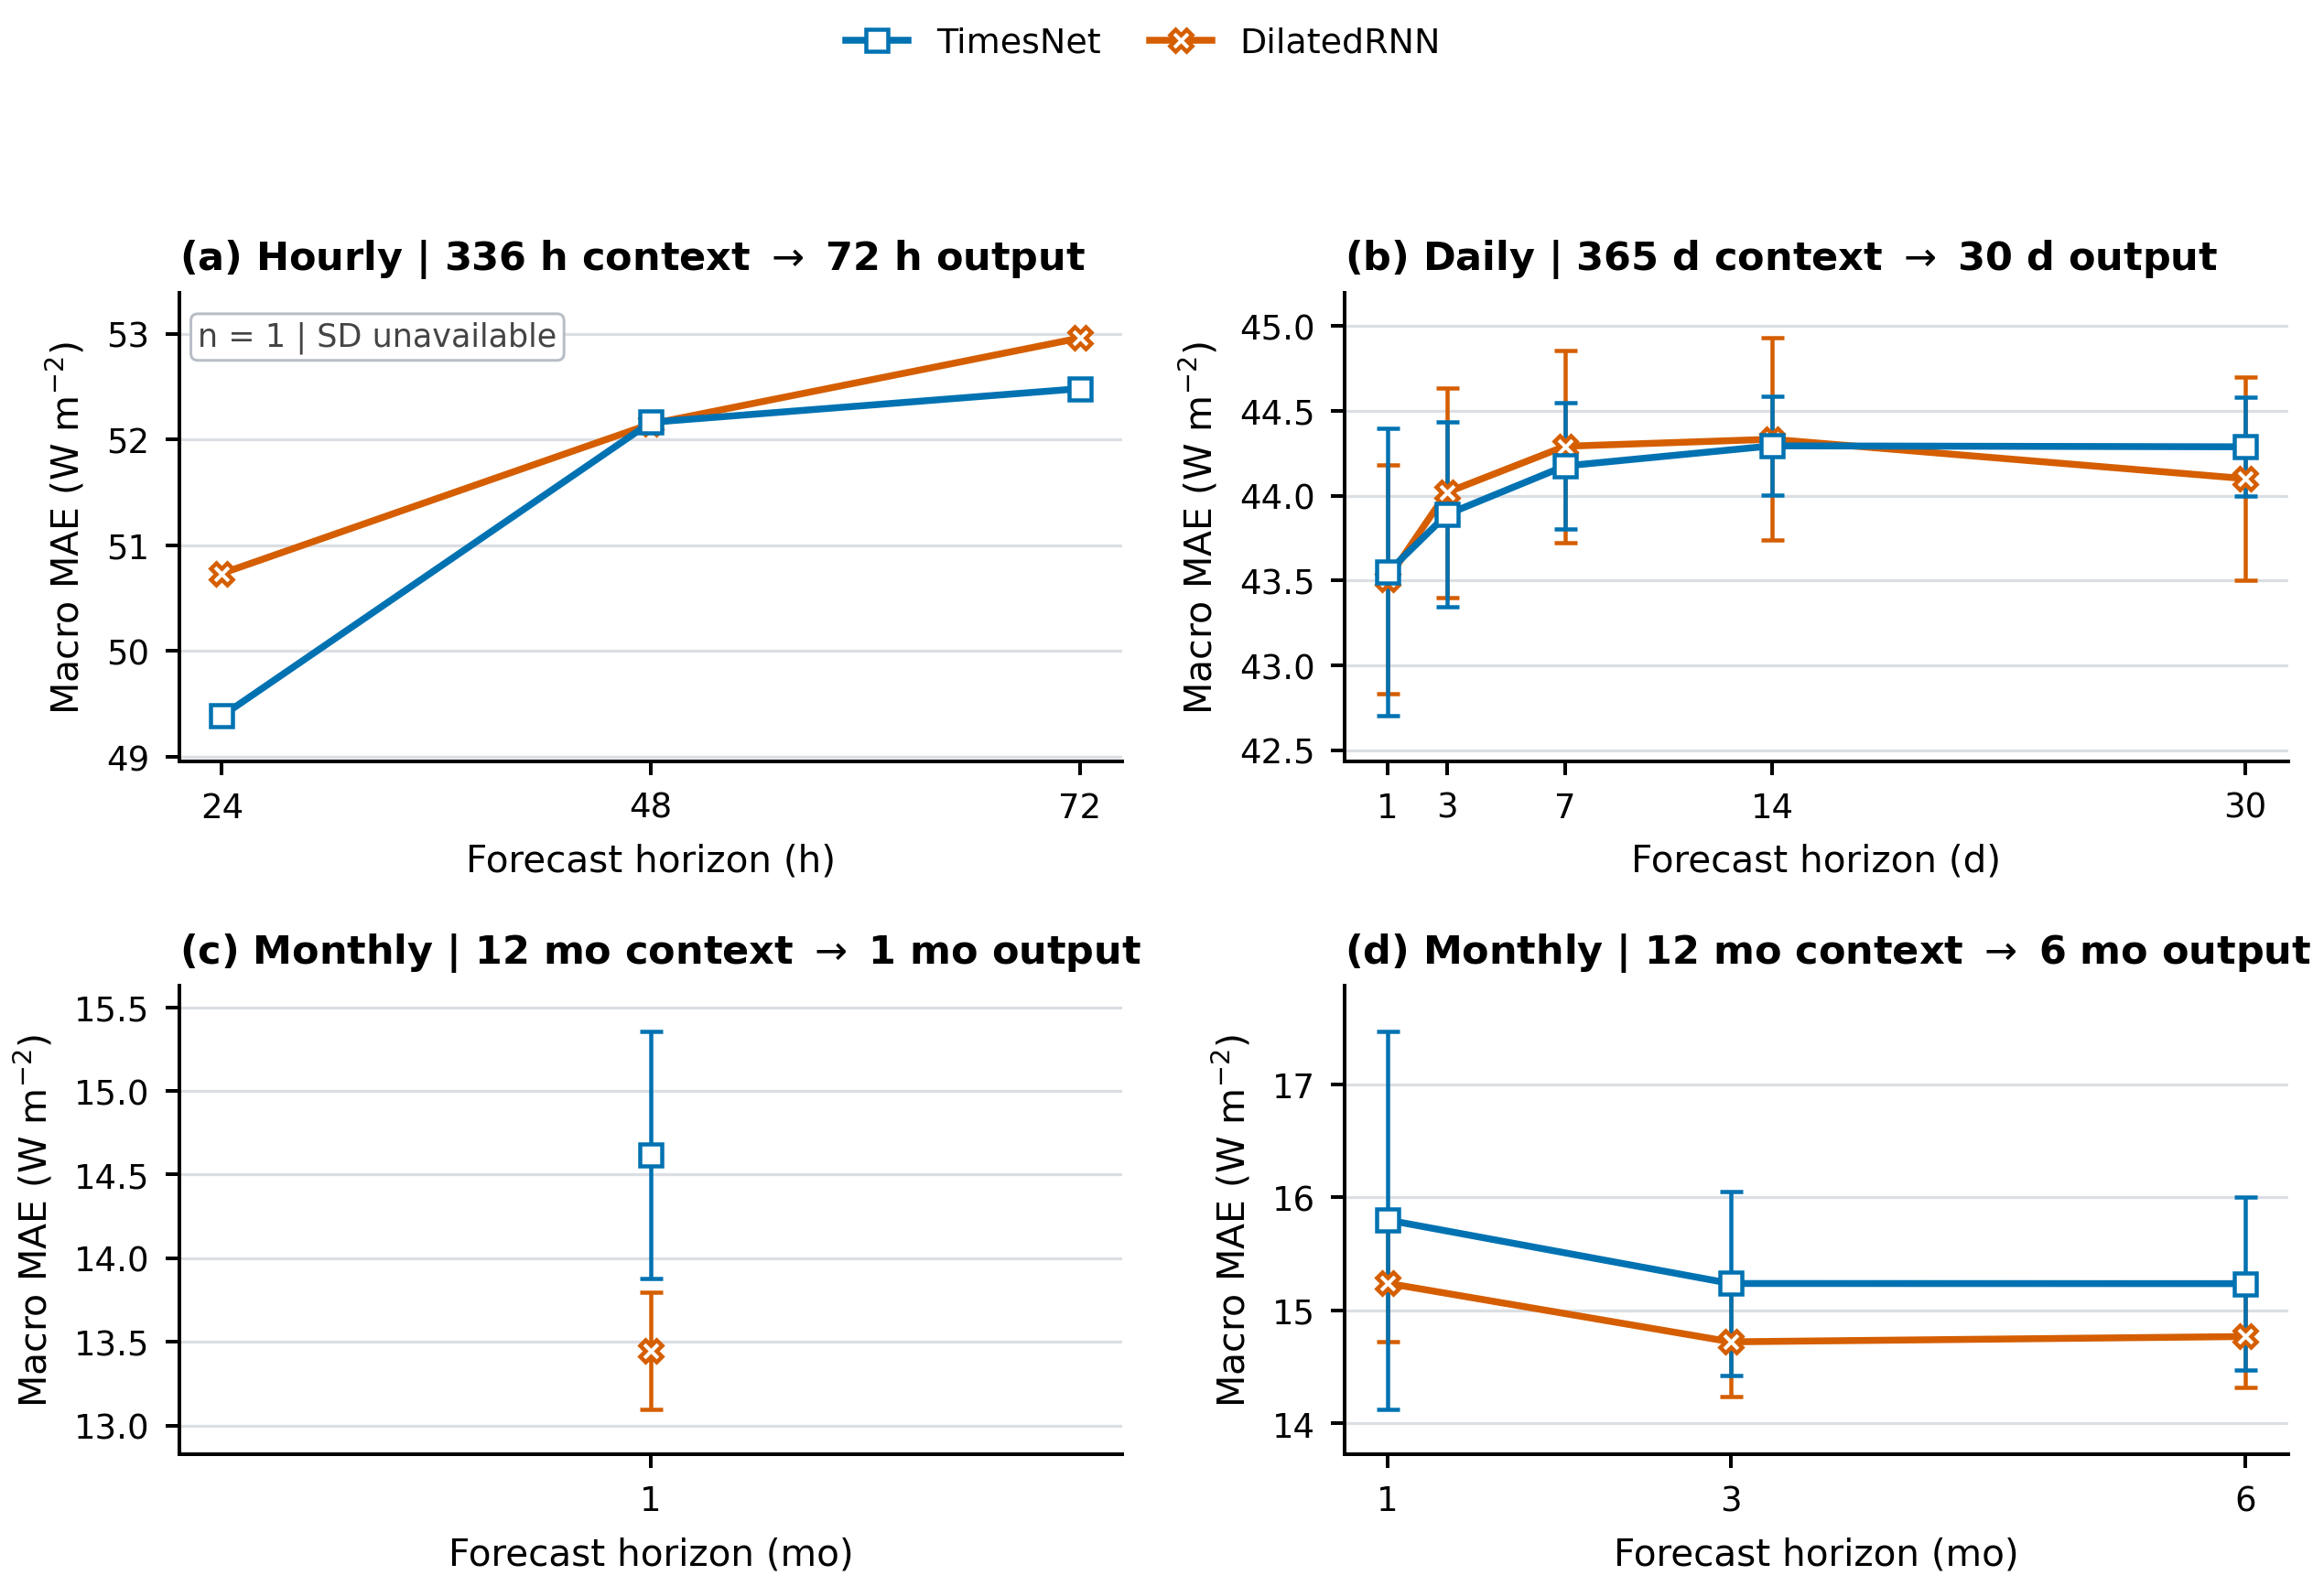
\includegraphics[width=\textwidth]{variabilidade_arquiteturas.png}
\caption{TimesNet and DilatedRNN seed-level macro-MAE: means with error bars
spanning one sample standard deviation. Color and marker shape identify
each architecture. The hourly extension is shown as $n=1$ without an error
bar. The full learned-model comparison is retained in the Supplementary Material.}
\label{fig:seed_variability}
\end{figure*}

\subsection{Reference benchmark and relation to the source protocols}
\label{sec:reference_benchmark}

The full benchmark remains necessary to interpret the focused comparison.
Supplementary Table S1 and Figure S1 retain every evaluated reference model
and cumulative checkpoint. XGBoost had the lowest macro-MAE at all hourly
checkpoints (50.50~W/m$^2$ at 72 hours) and at 1, 3, and 14 days.
LSTM led at 7 days (43.69~W/m$^2$), and DilatedRNN led at 30 days
(43.85~W/m$^2$), ahead of XGBoost (43.93~W/m$^2$).
Calendar climatology led both monthly tasks, with 12.57~W/m$^2$ at one month
and 13.03~W/m$^2$ over six months. Hourly climatology was not evaluated;
its missing entries are not zero errors. Consequently, a win over the other
focal architecture must not be read as a win over the entire benchmark.

The source studies motivate the hourly TimesNet and monthly DilatedRNN
contracts, but their original error values are not a matched comparison.
The present evaluation aligns inputs, origins, post-processing, aggregation,
and metrics within each task. Its ranking therefore uses the matched
predictions throughout, rather than combining results from the two
source protocols.

\subsection{Favorable and unfavorable cases}

The recorded global case rule selects the maximum and minimum, over all
available sites, origins, and declared cumulative horizons, of
$\mathrm{MAE}_{\mathrm{DilatedRNN}}-\mathrm{MAE}_{\mathrm{TimesNet}}$.
Figure~\ref{fig:contrasting_cases} plots both selected forecasts.
Weather is attached after selecting the error extremes. The largest TimesNet
gain occurred at GM Factory Zero for the 24-hour forecast beginning on
31 March 2024 in fixed local time: TimesNet and DilatedRNN obtained
45.43 and 109.90~W/m$^2$, respectively, a 64.47~W/m$^2$ advantage.
NASA POWER provided post-hoc context of 99.64\% mean cloud amount and
0.80~mm daily precipitation.

The largest deficit occurred at Tesla Gigafactory Texas for the 24-hour
forecast beginning on 28 March 2024: 150.02 versus 73.92~W/m$^2$, a
76.10~W/m$^2$ TimesNet disadvantage. NASA POWER reported 0.06~mm daily
precipitation and 2.14\% cloud amount; neither adverse-day threshold was
exceeded. An absent flag does not establish the absence of subdaily weather
variability. Both cases use the single hourly seed. Moreover, a global
selection based on raw MAE contrasts across resolutions can favor tasks
with larger absolute error scales. These examples cannot establish a
cross-resolution ranking or replace the complete aggregate evaluation.

\begin{figure*}[!t]
\centering
\includegraphics[width=\textwidth]{previsoes_casos_contrastantes.png}
\caption{Reference GHI and forecasts for the globally selected largest
TimesNet gain and deficit. Panels share a GHI scale. MAEs and descriptive
weather records refer to the selected 24-hour windows; meteorology was
joined only after case selection.}
\label{fig:contrasting_cases}
\end{figure*}

\subsection{Geographic and climatic interpretation}

Figure~\ref{fig:geographic_context} locates the ten sites in their descriptive
K\"oppen--Geiger context. With only ten purposively selected locations,
apparent differences between zones cannot establish a causal climatic effect.
Sites within a country can occupy distinct regimes, while nearby sites may
share correlated weather.

As an error-independent contextual example, the recorded meteorological
rule selected Hyundai Metaplant Georgia on 5 August 2024, with
82.66~mm/day corrected precipitation and 99.47\% cloud amount. This case
was selected without consulting either model's errors. Its meteorological
record is retained in the Supplementary Material, and its surrounding
forecast profiles are shown next.

\subsection{Multi-day irradiance profiles}
\label{sec:multiday_profiles}

Figure~\ref{fig:seven_day_profiles} extends the two error-selected cases
and the independent weather case to seven calendar days each: the event
date, three preceding days, and three following days. This fixed extension
rule does not optimize the displayed week using model errors. Each panel
contains 168 unique hourly targets and seven successive midnight forecast
origins. Only leads 1--24 of each 72-hour model output are retained; the
context advances daily while the fitted parameters remain fixed. The figure
therefore shows seven daily forecasts, not one 168-hour forecast.

Across these seven-day displays, TimesNet and DilatedRNN respectively
obtained MAEs of 99.73 and 115.07~W/m$^2$ at GM Factory Zero,
91.90 and 89.19~W/m$^2$ at Tesla Gigafactory Texas, and
109.42 and 122.98~W/m$^2$ at Hyundai Metaplant Georgia. These local
window errors are distinct from the single-event errors and the annual
macro-MAEs. The additional days reveal underprediction of some high-GHI
peaks and overprediction of low-GHI daytime periods by both architectures.
At the independently selected Georgia event, both forecasts exceed much
of the reference daytime profile. These trajectories expose limitations
of the GHI-only models, while the annual matched evaluation remains the
basis for declaring task-level winners.

\begin{figure*}[!t]
\centering
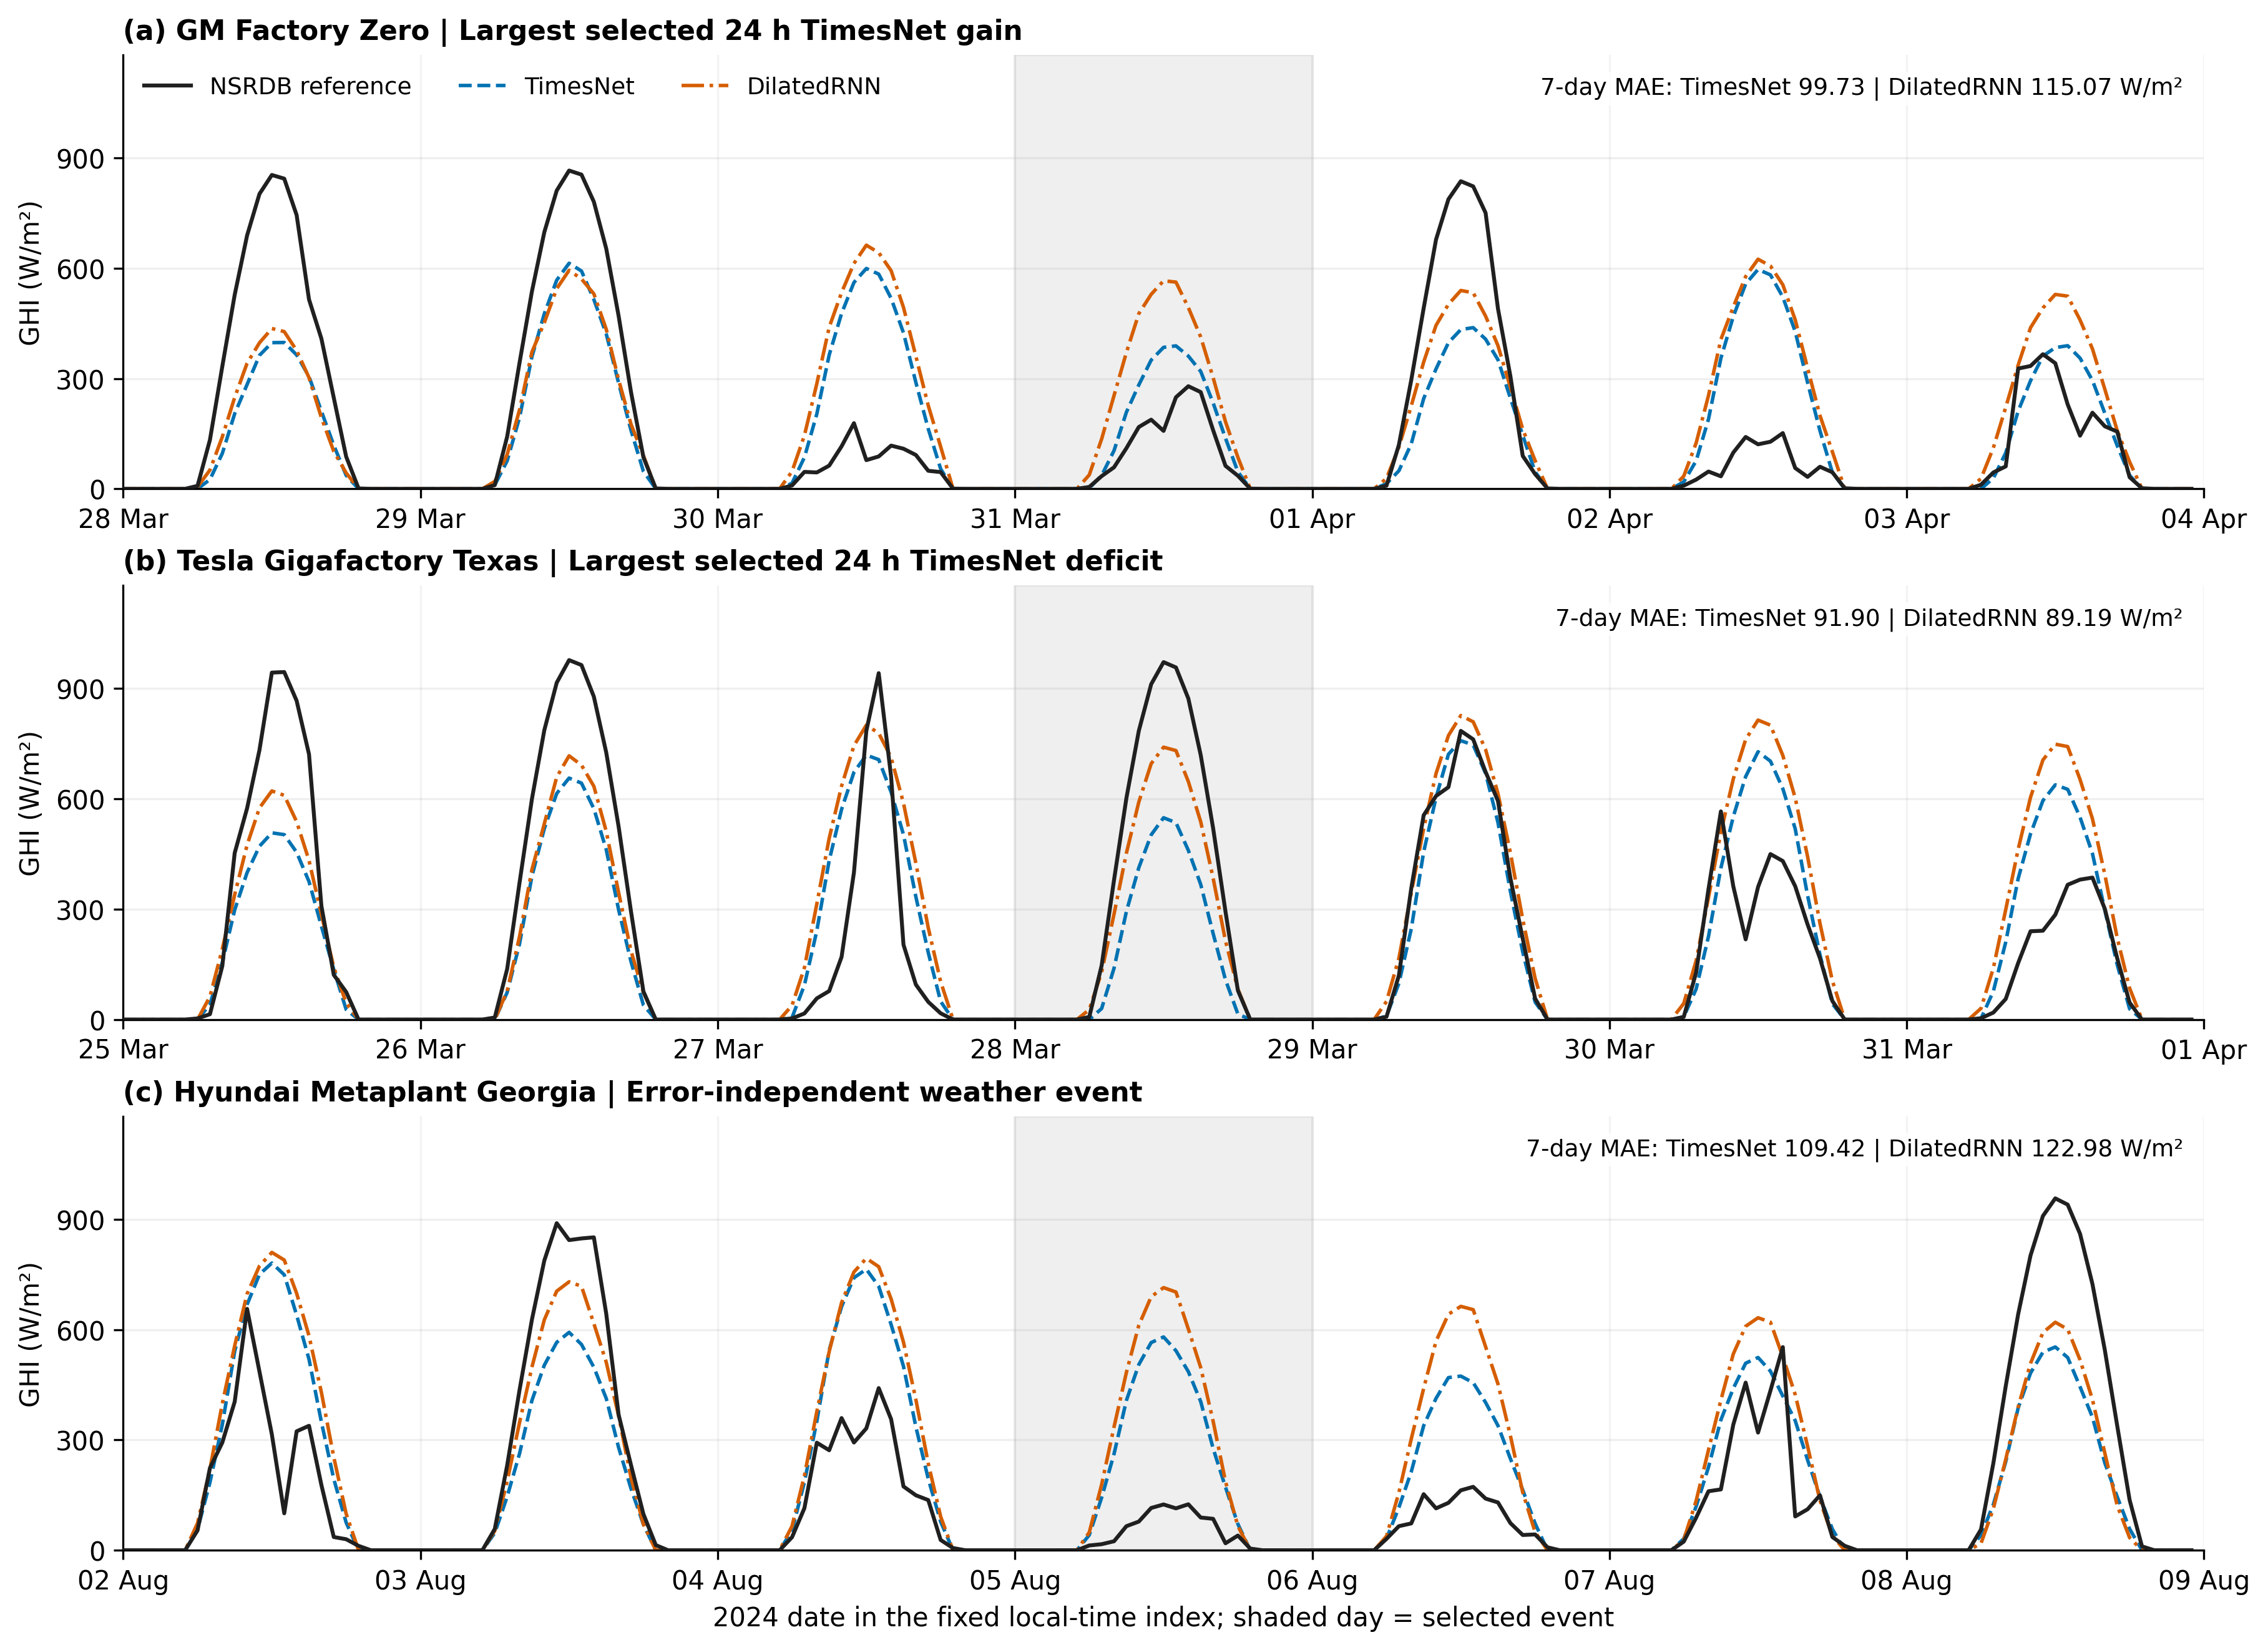
\includegraphics[width=\textwidth]{perfis_sete_dias.png}
\caption{Seven-day hourly GHI profiles around the two error-selected cases
and the error-independent NASA POWER event. Each curve joins seven
24-hour forecast prefixes issued on successive local midnights; it is not
a single seven-day forecast. Shading marks the original selected day.
MAEs use all 168 displayed targets per site, including nighttime; all
forecasts use seed 42 and the registered hourly post-processing.
Dates follow the fixed local-time index, and all panels share a GHI scale.}
\label{fig:seven_day_profiles}
\end{figure*}

\subsection{Threats to validity and limitations}
\label{sec:limitations}

\subsubsection{Construct and data validity}

NSRDB GHI is a satellite-informed physical-model estimate
\cite{sengupta2018}, not an on-site pyranometer record. Factory coordinates
select product grid cells, so neither the target nor its error quantifies the
irradiance at a particular roof surface. The purposive set of ten
factory-associated locations is also not a sample of factory electricity
demand, photovoltaic output, roof area, or operational constraints. The
industrial framing therefore identifies geographically relevant forecasting
sites; it does not establish plant-level energy savings.

The matched input contains only GHI available at the forecast origin and
site identity. This restriction controls predictor availability among learned
models, but excludes potentially useful weather information, such as cloud
motion, numerical weather predictions, and forecasts of aerosols and
temperature. A site embedding can also encode persistent
location-specific behavior and does not demonstrate transfer to an unseen
factory. Fixed local offsets produce regular hourly grids but do not reproduce
daylight-saving clock changes. Moreover, the daily/monthly archive was
retrieved independently of the hourly archive. The comparison across resolutions
therefore does not use controlled reaggregation of a single set of native
records.

\subsubsection{Temporal and statistical validity}

All test evidence is retrospective and restricted to 2024. It does not measure
prospective robustness under later satellite-product revisions, climate
nonstationarity, or new sites. The retrospective information set assumes
that each completed historical aggregate is immediately available; product
publication delays and operational data latency are not simulated. The
primary monthly task has only 48 pre-test refit origins per site, and the
exploratory six-month task has seven test origins per site. These small
samples limit the evidence available for fitting and evaluating monthly
models relative to the hourly and daily tasks.

Targets from adjacent multi-step origins overlap, creating strongly dependent
errors. Site-first aggregation avoids allowing that overlap to change spatial
weights, but it does not make the origins independent. The paired summaries
therefore use ten locations as descriptive units, without applying an
i.i.d. significance test to the overlapping target points. Nearby sites may
also share weather and model errors, so their summaries cannot be assumed
to be independent statistical replicates.

\subsubsection{Model-comparison validity}

TimesNet and DilatedRNN share inputs, origins, seeds, optimization limits, and
post-processing in the daily and monthly tasks, but their parameterizations and
inductive biases are not identical. The frozen configuration is a controlled
comparison rather than an exhaustive architecture-specific search. Moreover,
the hourly extension evaluates DilatedRNN using seed 42 against previously
generated comparator forecasts, whereas daily and monthly estimates use five
seeds. Comparisons across resolutions therefore reflect these protocol
differences, and seed variability cannot be assessed for the hourly task.
The reported TimesNet is a compact variant with sample-specific Fourier-period
selection; the findings do not establish a ranking of every implementation
bearing either architecture name.

Neural epoch selection minimizes normalized validation MSE, whereas the main
test ranking minimizes macro-MAE in W/m$^2$. These objectives weight errors
differently, and equal selection rules do not establish each model's best
achievable MAE. Calendar baselines also use explicit target calendar labels
and historical lookups unavailable as features to the learned models. Their
performance is a useful operational reference, but does not isolate
architecture under identical feature representations.

The neural parameter budgets also differ by task, as reported in
Table~\ref{tab:model_capacity}. Equal optimization rules do not imply equal
representational capacity, and the comparison cannot isolate whether a result
comes from recurrence, periodic convolution, parameter count, or their
interaction. Training and inference runtimes were not measured consistently
across runs, so the results do not support a hardware-efficiency ranking.

The zero floor enforces nonnegative predictions at all resolutions. The
additional hourly nighttime mask uses deterministic solar geometry, but no
common upper physical envelope is imposed. Consequently, implausibly high
daytime extrapolations remain reflected in the reported errors.

Hourly metrics retain all target hours after the common nighttime mask. Exact
nighttime zeros are part of the operational 72-hour trajectory, but they also
dilute the contribution of daylight errors to the all-hour average. The
reported hourly values must therefore be interpreted as full-trajectory
metrics. In particular, exact leads 24, 48, and 72 sample only the nighttime
23:00 intervals and cannot distinguish model skill in this experiment.
Daylight-only evaluation and complete lead profiles are needed to assess
the irradiance-producing hours separately.

\subsubsection{Contextual-data validity}

The K\"oppen--Geiger labels are climate classes extracted from cells of the
present nominal 1-km map \cite{beck2018}; they do not resolve microclimates within a cell or
conditions on a specific roof. Class boundaries are uncertain, as made explicit
by the 50\% confidence of the BMW San Luis Potos\'i assignment. Climate labels
are descriptive strata, not model inputs and not explanations of individual
forecast errors.

NASA POWER is likewise a gridded, model-based external product rather than
local rain-gauge or ceilometer evidence \cite{nasapowerdaily}. The 1~mm/day
precipitation and 80\% cloud thresholds provide reproducible post-hoc tags, but
thresholding cannot establish that weather caused a particular error.
These weather observations provide context for the selected cases, while
model rankings are based on the full aggregate evaluation.

\section{Conclusion}
\label{sec:conclusion}

The matched comparison shows that the relative performance of TimesNet and
DilatedRNN depends on the GHI forecasting task. Across ten factory-associated
locations, inputs available at the forecast origin, data partitions,
forecast origins, post-processing, metrics, and location weights were
controlled within each task. The results describe forecasts of the NSRDB solar resource, without
quantifying factory demand or photovoltaic output.

For cumulative macro-MAE, TimesNet led at 24 and 72 hours and at the daily
checkpoints up to 14 days. DilatedRNN led at 48 hours, 30 days, and in the
primary one-month task. In the exploratory six-month task, TimesNet led at
the one-month prefix, while DilatedRNN led at the three- and six-month
prefixes. Local win counts sometimes disagreed with the macro ranking:
DilatedRNN achieved lower terminal MAE at six of the ten sites in each of
the hourly, daily, and primary one-month tasks, and at seven sites in the
exploratory six-month task.

The complete benchmark puts these architecture-specific advantages in
perspective. XGBoost led all hourly checkpoints and the daily checkpoints
at 1, 3, and 14 days; LSTM led at seven days, and DilatedRNN led at 30 days
with 43.85~W/m$^2$, compared with 43.93~W/m$^2$ for XGBoost. Calendar
climatology led the monthly checkpoints. Neither TimesNet nor DilatedRNN
was consistently best across tasks.

Daily and monthly estimates use five-seed ensembles, and several differences
are small relative to the observed seed variability. The single hourly seed,
overlapping targets, one test year, and unequal parameter budgets limit
generalization. Post-hoc weather cases provide context but do not explain
model differences causally.

Future evaluation should include prospective years and unseen sites,
multiple hourly seeds, daylight-only metrics, measured computational cost,
and weather forecasts available at issuance. The matched protocol and
origin-level predictions provide a basis for testing these extensions.
Together, the task-level rankings, site-level differences, and reference
benchmarks show why architecture choice must be evaluated for the intended
forecasting task.


\section*{Acknowledgments}
The authors acknowledge financial support from FAPEMIG (grant OET-00243-26).

\section*{Declaration of Competing Interest}
The authors declare that they have no known competing financial interests or
personal relationships that could have appeared to influence the work
reported in this article.

\section*{Data and Code Availability}
Source code and protocol definitions are maintained at
\url{https://github.com/enggusttavomn/TCC}.
The comparisons reported here use the corrected multi-resolution archive
identified in the Supplementary Material. That full forecast bundle is not
included in the current public repository snapshot; access to it is required
to reproduce the reported metrics from individual predictions.
External NSRDB, K\"oppen--Geiger, and NASA POWER products remain subject to
their respective providers' access and licensing conditions.

\bibliographystyle{elsarticle-num}
\bibliography{references}

\end{document}
